\documentclass[12pt]{article}
\usepackage[utf8]{inputenc}
\usepackage[T1]{fontenc}
\usepackage[top=0.60in, bottom=0.80in, left=0.60in, right=0.60in]{geometry}
\usepackage{graphicx}
\usepackage{siunitx}
\usepackage{listings}
\usepackage{amsmath}
\usepackage[labelfont=bf]{caption}

\newcommand{\Msun}{\,\mathrm{M_{\odot}}}
\newcommand{\Rsun}{\,\mathrm{R_{\odot}}}
\newcommand{\MWD}{M_{\mathrm{WD}}}
\newcommand{\Mstar}{M_{\star}}
\newcommand{\alphace}{\alpha_{\mathrm{CE}}}
\newcommand{\alphath}{\alpha_{\mathrm{th}}}
\newcommand{\alpharec}{\alpha_{\mathrm{rec}}}
\newcommand{\Ebind}{E_{\mathrm{bind}}}
\newcommand{\Egrav}{E_{\mathrm{grav}}}
\newcommand{\Eint}{E_{\mathrm{int}}}
\newcommand{\Eth}{E_{\mathrm{th}}}
\newcommand{\Erec}{E_{\mathrm{rec}}}
\newcommand{\Porb}{P_{\mathrm{orb}}}
\newcommand{\au}{\, \mathrm{au}}

\title{Wide Post-Mass Transfer White-Dwarf Binaries}
\author{Runqiu Ye}
\date{June, 2024}

\begin{document}

\maketitle

\section{Introduction} \label{sec:intro}

Common envelope (CE) is the outcome of unstable mass transfer. During CE, both stars orbit inside an envelope and spiral inward. If the energy liberated in this process is enough to eject the CE, then the result of CE process is a close binary. If, on the contrary, the liberated energy is not enough to eject the envelope, then the result of the process is a merger. In observation results, a number of WD+MS binaries are wider than expected, and CE is expected to be the main channel to form these white dwarf binaries \cite{yamaguchi_hi, yamaguchi_lo}. In the MESA model utilized by \cite{yamaguchi_hi, yamaguchi_lo}, wide post-CE WD+MS binaries can be formed in a certain range of initial separation with only gravitational and internal energy included in the calculation. 

In this paper, we are going to explore the formation possibility of these wide post-mass transfer WD+MS binaries with COSMIC model. We perform COSMIC simulation on both individual binary star systems and sampled population to explore the formation of WD+MS binaries under different conditions. In section \ref{sec:ce}, we are going to investigate formation of individual wide WD+MS binaries through CE for a variety of variables, including initial mass, initial separation, CE efficiency, and the energy budget of the CE. In section \ref{sec:stable}, we are going to explore the formation of individual wide WD+MS binaries through stable mass transfer. In section \ref{sec:population}, we will research on how different COSMIC model affect simulation results of a sample population of binary star systems, and how the formation of post WD+MS binaries depends on various parameters.

Throughout the paper, the stellar type and evolution type follows the BSE conventions. \verb|kstar| values specify the evolutionary state of the star, and \verb|evol_type| values specify the evolutionary changes of the binary systems:

\begin{tabular}{|cl|cl|}
  \hline
  \verb|kstar| & \textbf{evolutionary state} & \verb|evol_type| & \textbf{evolutionary change} \\
  \hline
  0 & MS $<0.7 \Msun$ & 1 & initial state \\
  1 & MS $>0.7 \Msun$ & 2 & kstar change \\
  2 & Hertzsprung Gap & 3 & begin Roche lobe overflow\\
  3 & First Giant Branch & 4 & end Roche lobe overflow\\
  4 & Core Helium Burning & 5 & contact \\
  5 & Early AGB & 6 & coalescence \\
  6 & TP-AGB & 7 & begin common envelope \\
  7 & Naked Helium Star MS & 8 & end common envelope \\
  8 & Naked Helium Star Hertzsprung Gap & 9 & no remnant leftover \\
  9 & Naked Helium Star Giant Branch & 10 & max evolution time \\
  10 & Helium White Dwarf & 11 & binary disruption \\
  11 & Carbon/Oxygen White Dwarf & 12 & begin symbiotic phase \\
  12 & Oxygen/Neon White Dwarf & 13 & end symbiotic phase \\
  13 & Neutron Star & 14 & blue straggler \\
  14 & Black Hole & 15 & supernova of primary \\
  15 & Massless Remnant & 16 & supernova of secondary \\
  \hline
\end{tabular}

\section{Formation Through Common Envelope} \label{sec:ce}
In \cite{yamaguchi_hi, yamaguchi_lo}, the author discussed the formation of WD+MS binaries through CE for both high-mass and low-mass systems, and it was found that wide WD+MS systems can be formed for certain energy budgets and certain initial separation in the MESA model. We hope to explore similar models in COSMIC.

In \cite{yamaguchi_hi, yamaguchi_lo}, to explore the dependency of the final separation $a_f$ in the post-CE binary on the initial separation $a_i$ in the pre-MT binary, the author first ran a stellar evolution model of the primary star using MESA. Its evolution up to AGB phase is followed. With the model, the binding energy of the CE is calculated as

\begin{equation}
  E_{\mathrm{bind}} = E_{\mathrm{grav}} + E_{\mathrm{int}} = \int_{M_{\mathrm{core}}}^{M_{\mathrm{tot}}} -\frac{Gm}{r(m)} + U(m) dm,
  \label{budget-int}
\end{equation}
or
\begin{equation}
  E_{\mathrm{bind}} = E_{\mathrm{grav}} + \alphath E_{\mathrm{th}} + \alpharec E_{\mathrm{rec}}.
  \label{budget-th-rec}
\end{equation}
After that, the change of separation through CE evolution is calculated using
\begin{equation}
  E_{\mathrm{bind}} = \alphace \left(-\frac{G\MWD \Mstar}{2a_f}+\frac{GM_i \Mstar}{2a_i}\right).
  \label{ebind-sep}
\end{equation}

In COSMIC, the CE is modeled using a structural parameter $\lambda$, where
\begin{equation}
  \Ebind = \frac{G M_i M_{\mathrm{env}}}{\lambda R_i}.   
  \label{ebind}
\end{equation}
This $\lambda$ is represented in COSMIC as the \verb|lambdaf| flag in \verb|BSEDict|. To compare MESA model with COSMIC, we intend to compare how the energy budget utilized in past papers matches with the CE model in COSMIC. We approach this by calculating the effective $\lambda$ value for each of the common envelope energy budget used in \cite{yamaguchi_hi, yamaguchi_lo}. 

\subsection{High Mass Systems $(7 \Msun + 1 \Msun)$} \label{subsec:high}

\subsubsection{Methods and results}

According to \cite{yamaguchi_hi}, the lower limit of WD mass $M_{\mathrm{MD, min}}$ in the observational sample is calculated to be $1.244\Msun \sim 1.418\Msun$. The corresponding mass of MS progenitor is expected to be in the range of $6 \sim 9 \Msun$, and the companion mass has median around $1\Msun$. MESA results for $7\Msun + 1\Msun$ systems is documented in \cite{yamaguchi_hi}. Hence, we also consider a $7\Msun + 1\Msun$ evolution model in COSMIC and compare the results with those in \cite{yamaguchi_hi}.

We ran COSMIC binary evolution simulation of a $7\Msun + 1\Msun$ system and investigate how the final separation $a_f$ depends on the initial separation $a_i$ and the CE parameter $\lambda$. The initial separation is a linear grid in range $2 \sim 8 \au$ with $400$ points. The CE flag \verb|lambdaf| is a linear grid in range $0 \sim -100$ with $2000$ steps, which corresponds to $0 \sim 100$ for CE parameter $\lambda$. Also, we ran these parameters with four different CE efficiencies — $\alphace = 1$, $\alphace = 0.9$, $\alphace = 0.6$, and $\alphace = 0.3$, the same as recorded in \cite{yamaguchi_hi}. In total, for each of the $4$ different CE efficiency $\alphace$, we ran a grid of $80000$ binary star systems with different initial separation $a_i$ and CE parameter $\lambda$.

After simulation is finished, we select the time-step when the system finished CE for the first time (\verb|evol_type = 8|). At this moment, if the system is a WD+MS system, we record their separation as the final separation $a_f$. Otherwise, we set $a_f = 0$ and consider this initial condition unable to produce a WD+MS system. We create four heat maps for the four different CE efficiencies. In Figure \ref{res_hi}, we plot the final separation $a_f$ of the WD+MS systems against initial separation $a_i$ and the CE flag $- \lambda$.

\begin{figure}
  \centering
  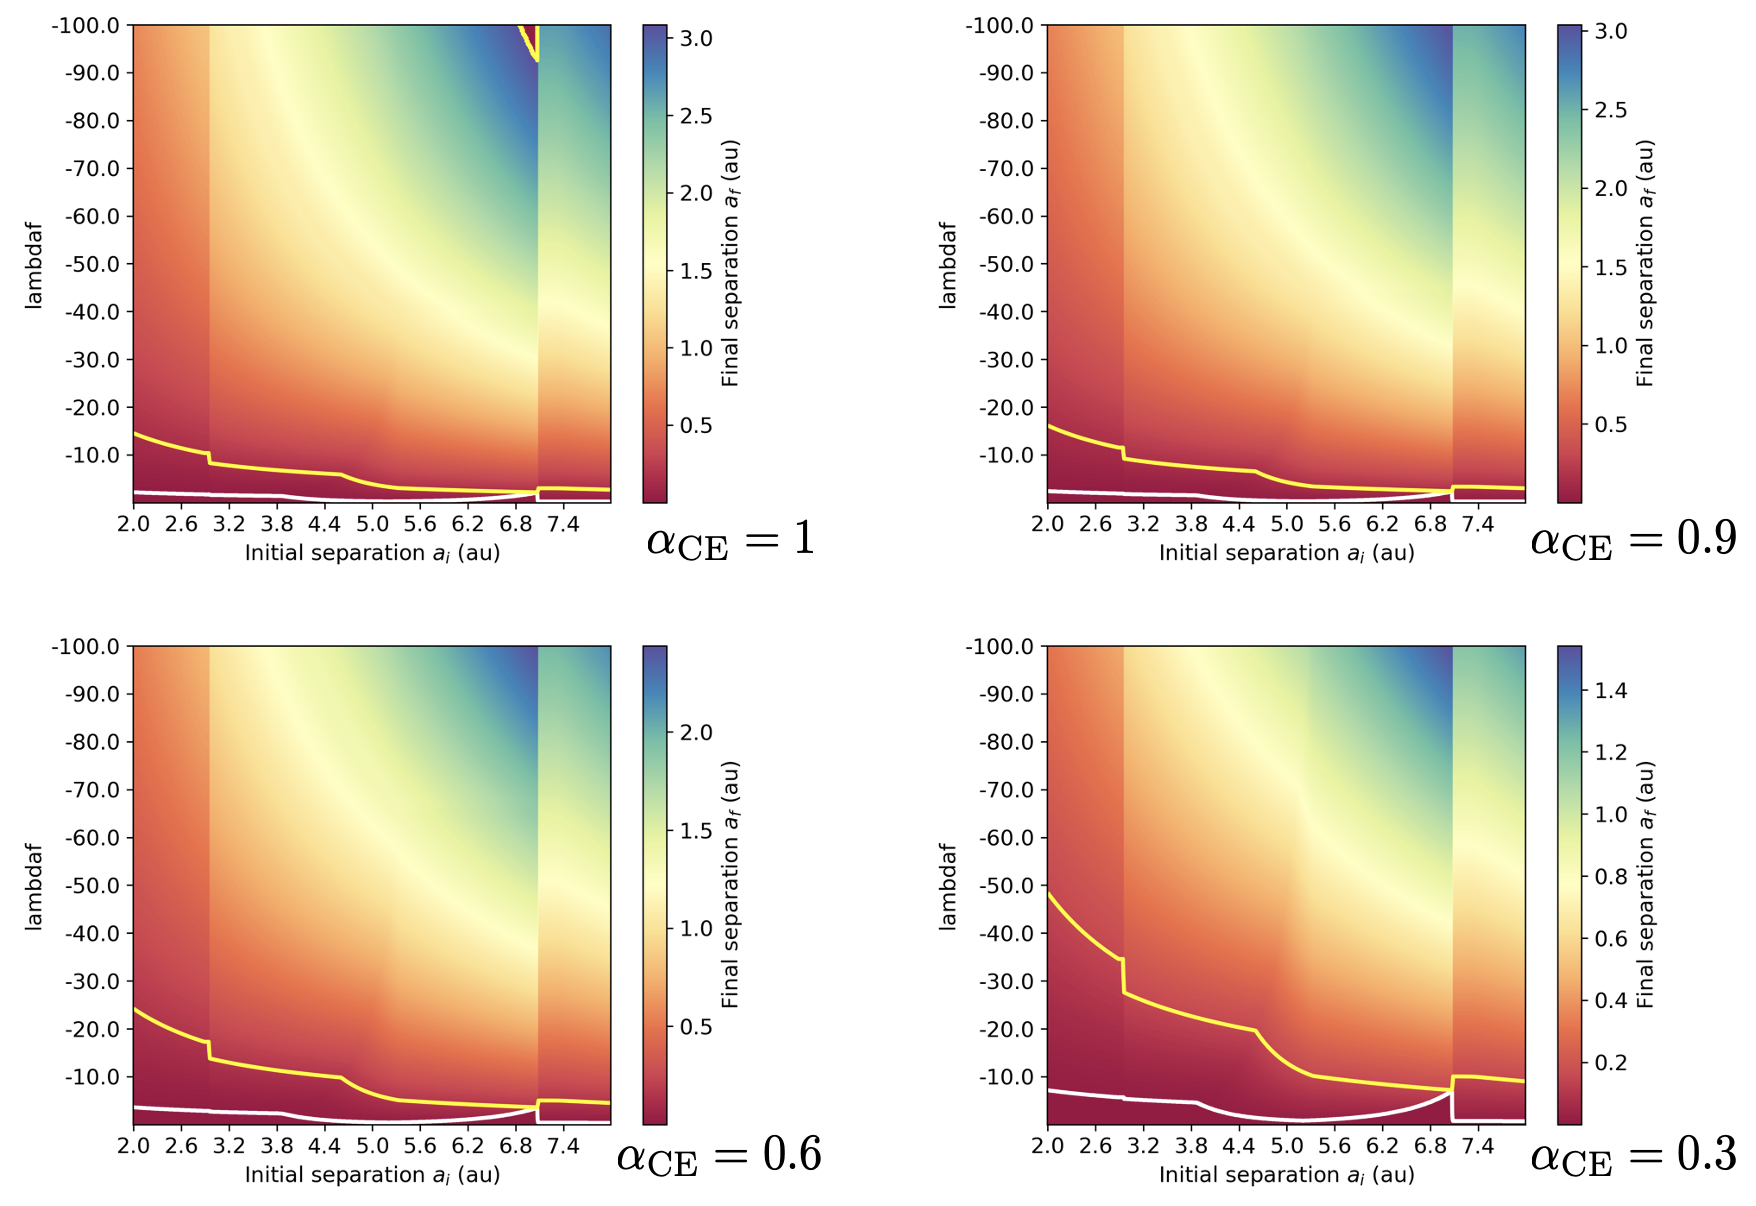
\includegraphics[width=\linewidth]{fig/7+1results.png}
  \caption{Heat map of final separation $a_f$ against initial separation $a_i$ and CE flag $-\lambda$. Different panels represent four different CE efficiencies $\alphace = 1$, $0.9$, $0.6$, and $0.3$. The white and yellow contour corresponds to $a_f = 0.01 \au$ and $a_f = 0.15 \au$ respectively. WD+MS binaries is not possible for separation smaller than $0.01 \au$, and $0.15 \au$ is the minimum separation of wide WD+MS binaries in observational results. Outside the white contour no desired system forms.}
  \label{res_hi}
\end{figure}

\subsubsection{Discussions}

A typical change of \verb|evol_type| through the evolution is $\boxed{\text{\textbf{*-3-7-8-4-*-3-7-8-4-*}}}$ (refer to Section \ref{sec:intro} for correspondence between \verb|evol_type| and evolutionary changes), where WD+MS is reached during the second mass transfer process. Another possible change of \verb|evol_type| through the volution is $\boxed{\text{\textbf{*-3-7-8-7-8-4-*}}}$. It is worth noting that most of these systems experience two mass transfer phases in COSMIC before reaching WD+MS. That is, during the evolution process, two CE processes take place, between which there is a period of time. Statistically, we found that \textbf{(***TO-DO***)} fraction of all our $320000$ simulated binaries experience two CE processes before reaching WD+MS. To explain this qualitatively, we notice that when the primary loses too much mass during the first CE, the CE process ends, as the radius of the primary becomes smaller than the Roche lobe. After the primary fills its Roche lobe and has a large enough envelope again, the CE process resumes and causes two CE processes in total.

There are several interesting points of the results. First of all, comparing the four panels, we found that as $\alphace$ decreases, the final separation decreases in general. This can be explained by Equation \ref{ebind-sep}. Qualitatively, note that more energy from the orbit is needed to eject the envelope for low $\alphace$, so the resulting $a_f$ is expected to be smaller. 

From Figure \ref{res_hi}, we also notice that final separation $a_f$ jumps obviously at about $2.9 \au$, and $7.1 \au$. After investigating the \verb|bpp| array of these simulations, we find out the jump at about $2.9 \au$ and $7.1 \au$ is likely due to the difference of \verb|kstar_1| at the start of RLOF. For $a_i < 2.9 \au$, RLOF starts when \verb|kstar_1 = 3|. For $a_i = 2.9 \au$, RLOF starts when \verb|kstar_1 = 4|. For $2.9 \au < a_i < 7.1 \au$, RLOF starts when \verb|kstar_1 = 5|. For $a_i > 7.1 \au$, RLOF starts when \verb|kstar_1 = 6|. For different star type, the structure and mass of the envelope is different, leading to different binding energy $\Ebind$ and thus different final separation $a_f$.

\begin{figure}
  \centering
  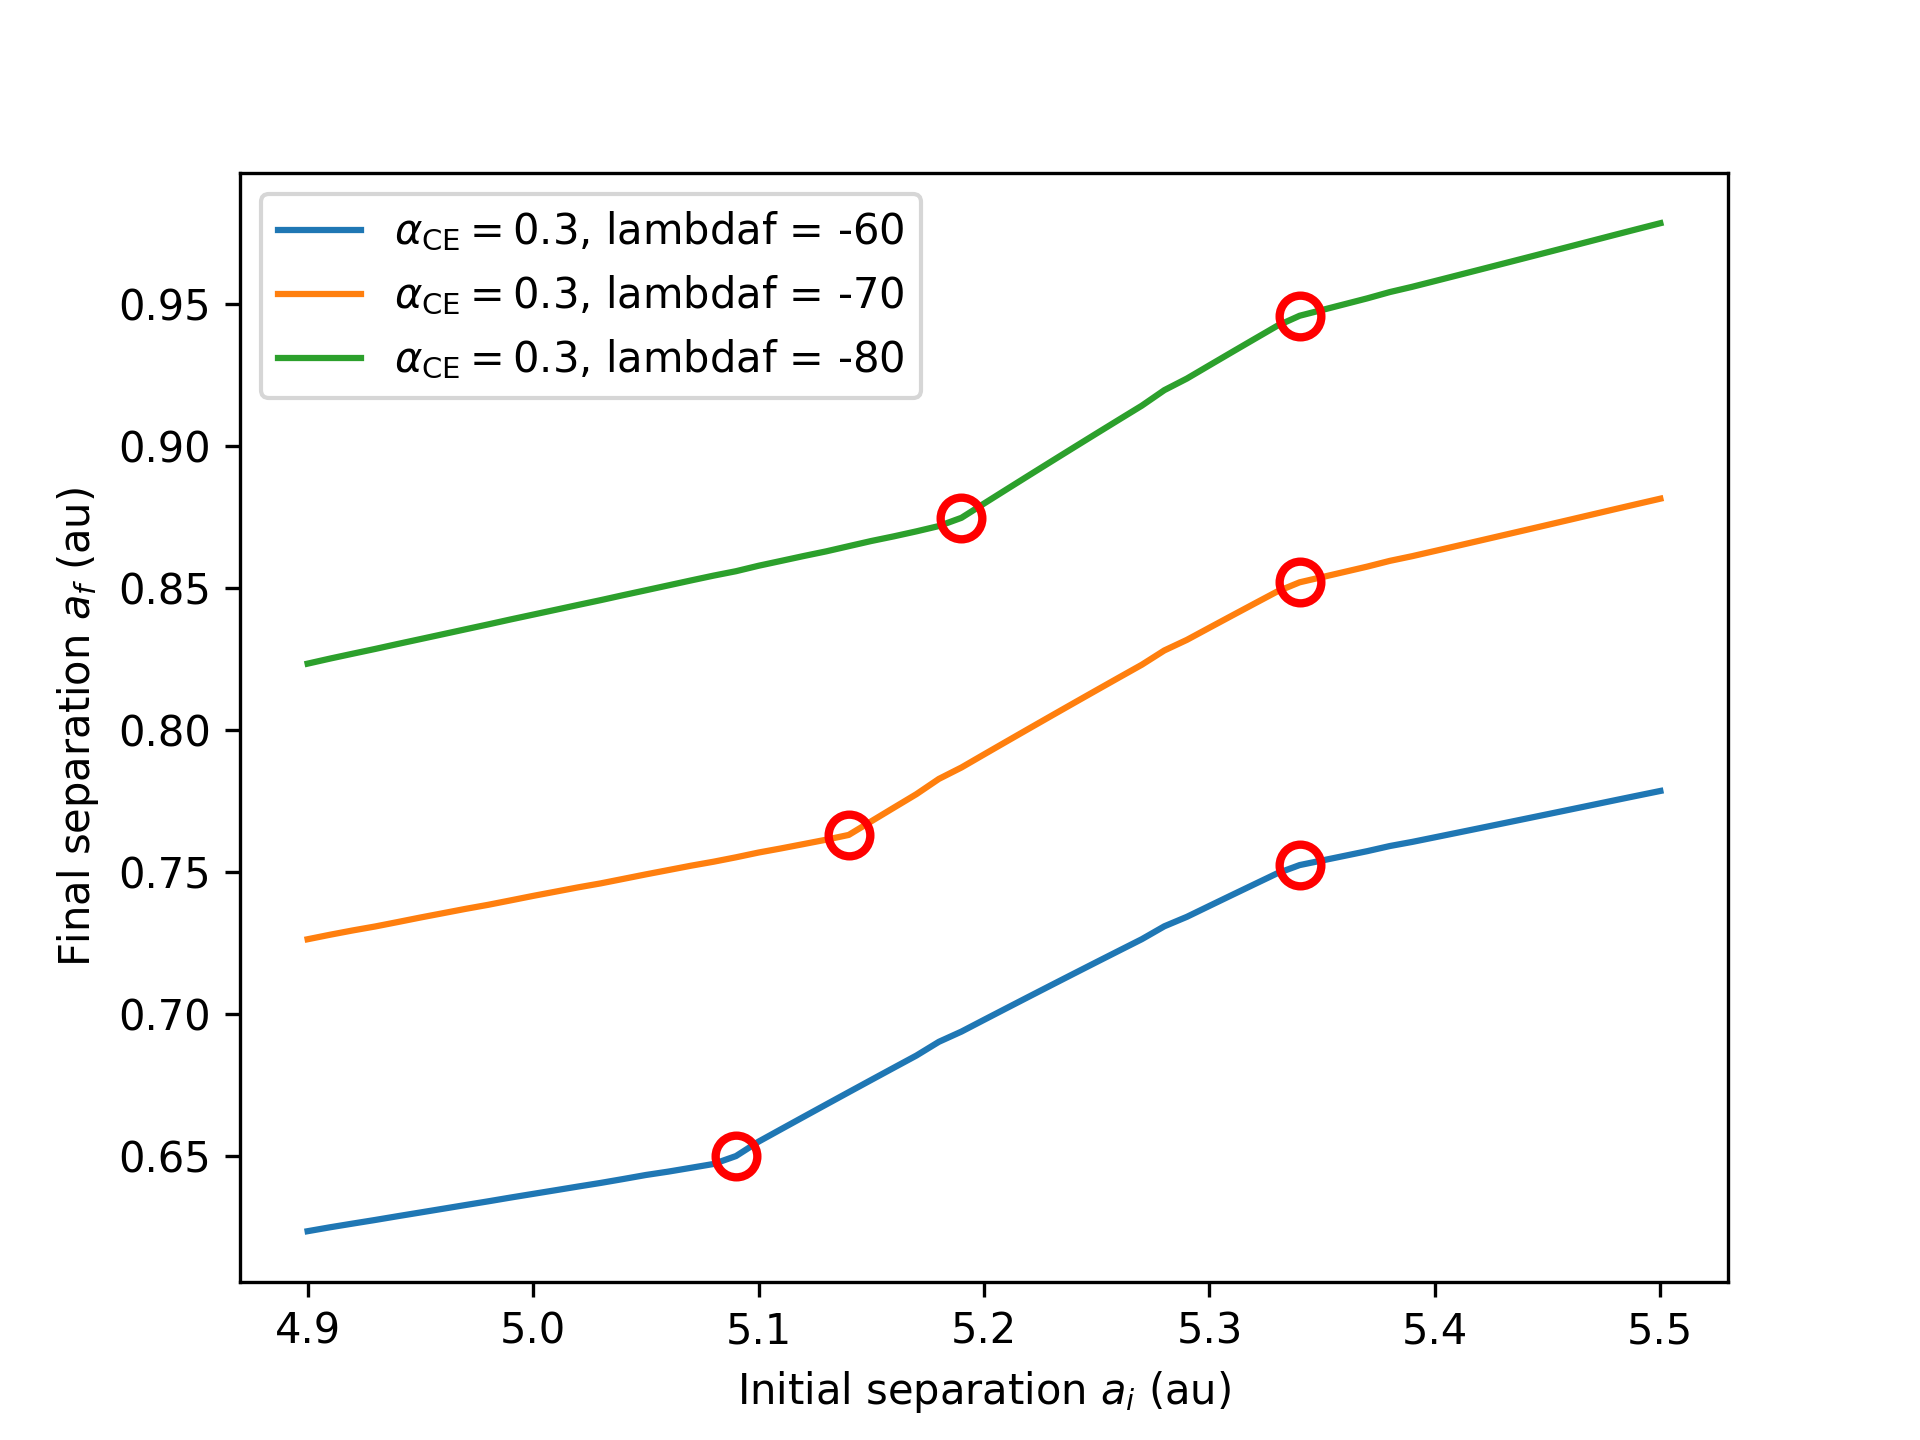
\includegraphics[width = 0.6\linewidth]{fig/jump-zoom.png}
  \caption{Dependence of final separation $a_f$ on initial separation $a_i$ for $\alphace = 0.3$. Simulation results of $\lambda_f = 60$, $70$, and $80$ are shown. The red circles emphasizes the jump of final separation as initial separation increases.}
  \label{jump-zoom}
\end{figure}

Inspecting more closely, we found that the final separation $a_f$ jumps at about $5.2 \sim 5.4 \au$. This is especially obvious with $\alphace = 0.3$. To illustrate, we zoom in the simulation results of $\alphace = 0.3$, and present the change of final separation $a_f$ as initial separation $a_i$ increases in Figure \ref{jump-zoom}. From here, we can clearly see two jumps — one between $5.1\au$ and $5.2\au$, the other at $5.34\au$. To explain this, we again go to the \verb|bpp| array of these systems. The first jump is because the evolution process changes from $\boxed{\text{\textbf{3-7-8-4-3-7-8-4}}}$ to $\boxed{\text{\textbf{3-7-8-7-8-4}}}$. This means that for relatively larger initial separation $a_i$, the primary fills its Roche lobe all the time, leading to more mass loss during a shorter timescale and thus larger final separation. For the second jump, it is because \verb|kstar_1| changes from \verb|8| to \verb|9| at the start of the second common envelope. This changes the binding energy of the common envelope and thus changes the final separation.

Finally, notice that there exists a small triangular gap in the figure for $\alphace = 1$. This is because \verb|kstar_1| becomes a neutron star and no rows in the \verb|bpp| gets selected.

In conclusion, with a large $\lambda$, it is possible to create wide post-mass transfer WD+MS systems with final separation $a_f > 0.15 \au$, which is the minimal separation of our observed objects. In next section, we will compare these results with default settings in COSMIC and with results in \cite{yamaguchi_hi}, in order to investigate the possibility of forming wide WD+MS systems through CE.

\subsubsection{Comparison}
After we have obtained the simulation results for different initial conditions, now we can calculate the effective $\lambda$ that matches with results in \cite{yamaguchi_hi}. For each fixed initial separation $a_i$, we loop through the COSMIC results with the same initial separation, and find the $\lambda$ value that results in a final separation closest to MESA model results. We record this $\lambda$ as the effective $\lambda$ that matches the binding energy formalism at initial separation $a_i$.

\begin{figure}
  \centering
  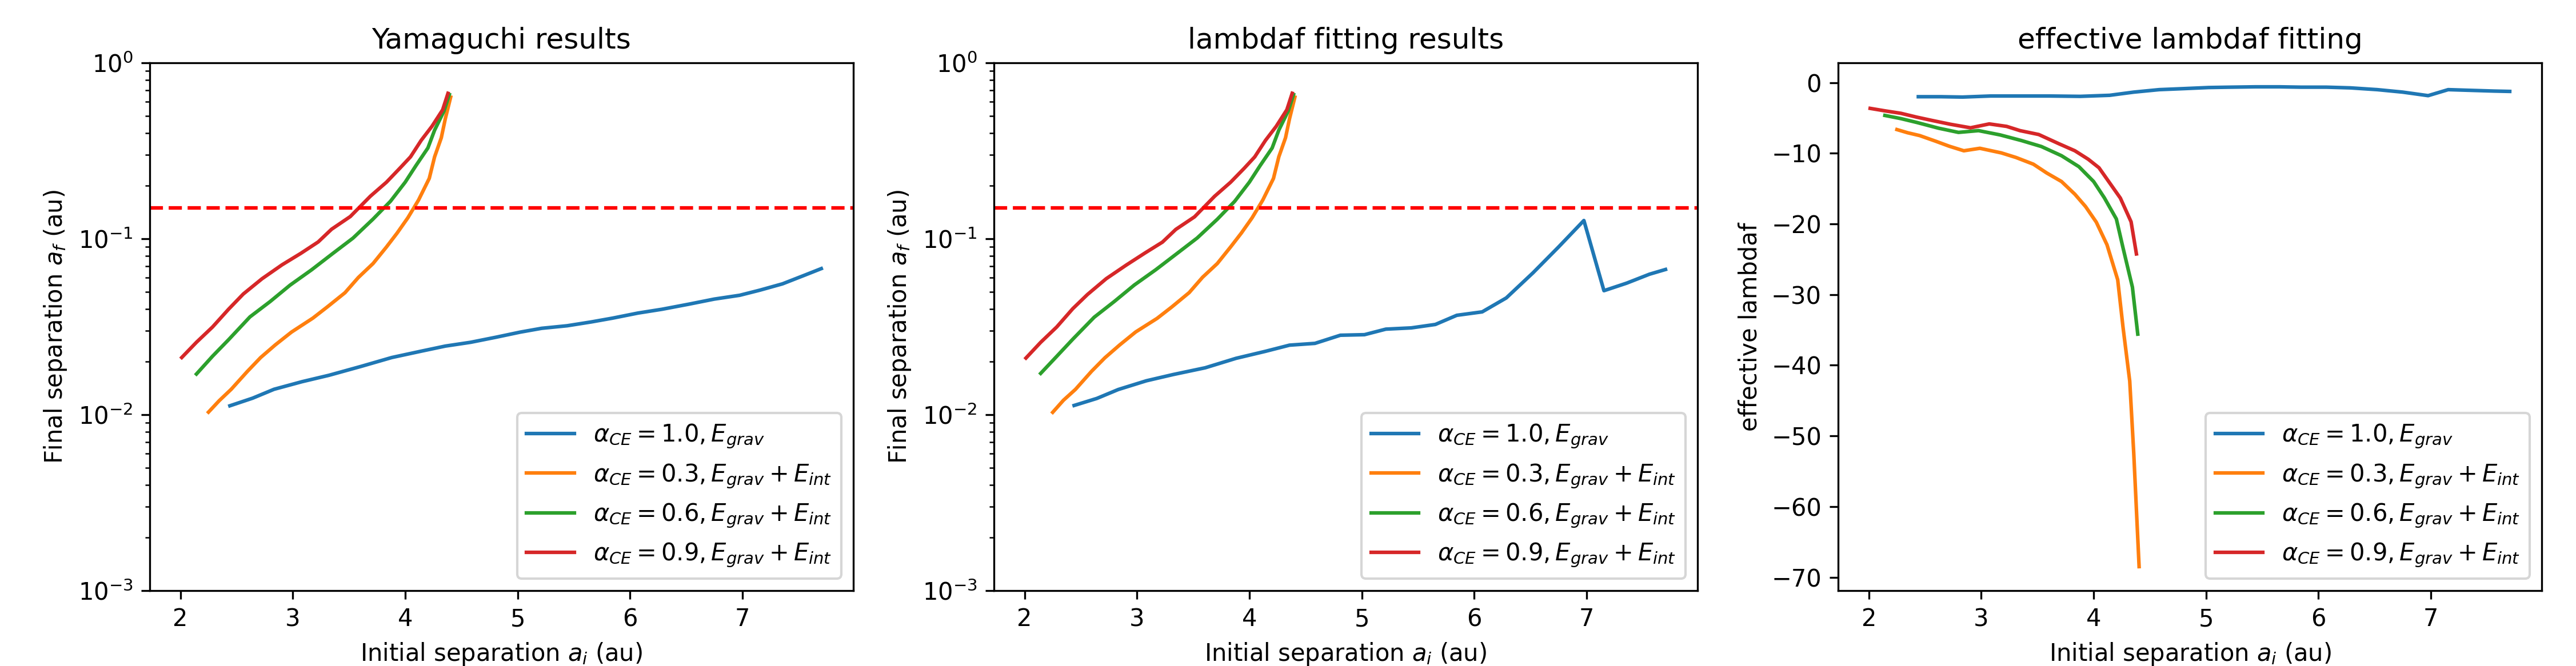
\includegraphics[width=\linewidth]{fig/7+1fit.png}
  \caption{Effective $\lambda$ fitting results of a $7\Msun + 1\Msun$ system for common envelope structure in MESA. Different lines represent different $\alphace$ and different common envelope energy budget, as shown in the legend. Left panel: recreation of MESA results in \cite{yamaguchi_hi} of how final separation $a_f$ depends on initial separation $a_i$. Central panel: COSMIC results of how final separation $a_f$ depends on initial separation $a_i$, produced by the effective $\lambda$ calculated. Right panel: effective $\lambda$ in COSMIC that corresponds to the MESA results for each initial separation $a_i$. The red dashed line in the left and middle panel represents $0.15 \au$, which is the minimal separation for observed wide post-CE WD+MS binaries.}
  \label{fit_hi}
\end{figure}

We present the fitting results for energy budget $\Ebind = \Egrav + \Eint$ in Figure \ref{fit_hi}. Notice that in the central panel, there is a small bump of the blue line. This is because at $6 \sim 7 \au$, we cannot reach such low final separation in COSMIC while forming a WD+MS binary at the same time. From the left panel, we can see that it is possible to create WD+MS binaries with $a_f > 0.15 \au$ in MESA as long as internal energy $\Eint$ is included, with initial separation $a_i > 3.5 \au$. However, in the right panel we show that this correspond to very large $\lambda$ in COSMIC ($\lambda > \sim 20$).

\begin{figure}
  \centering
  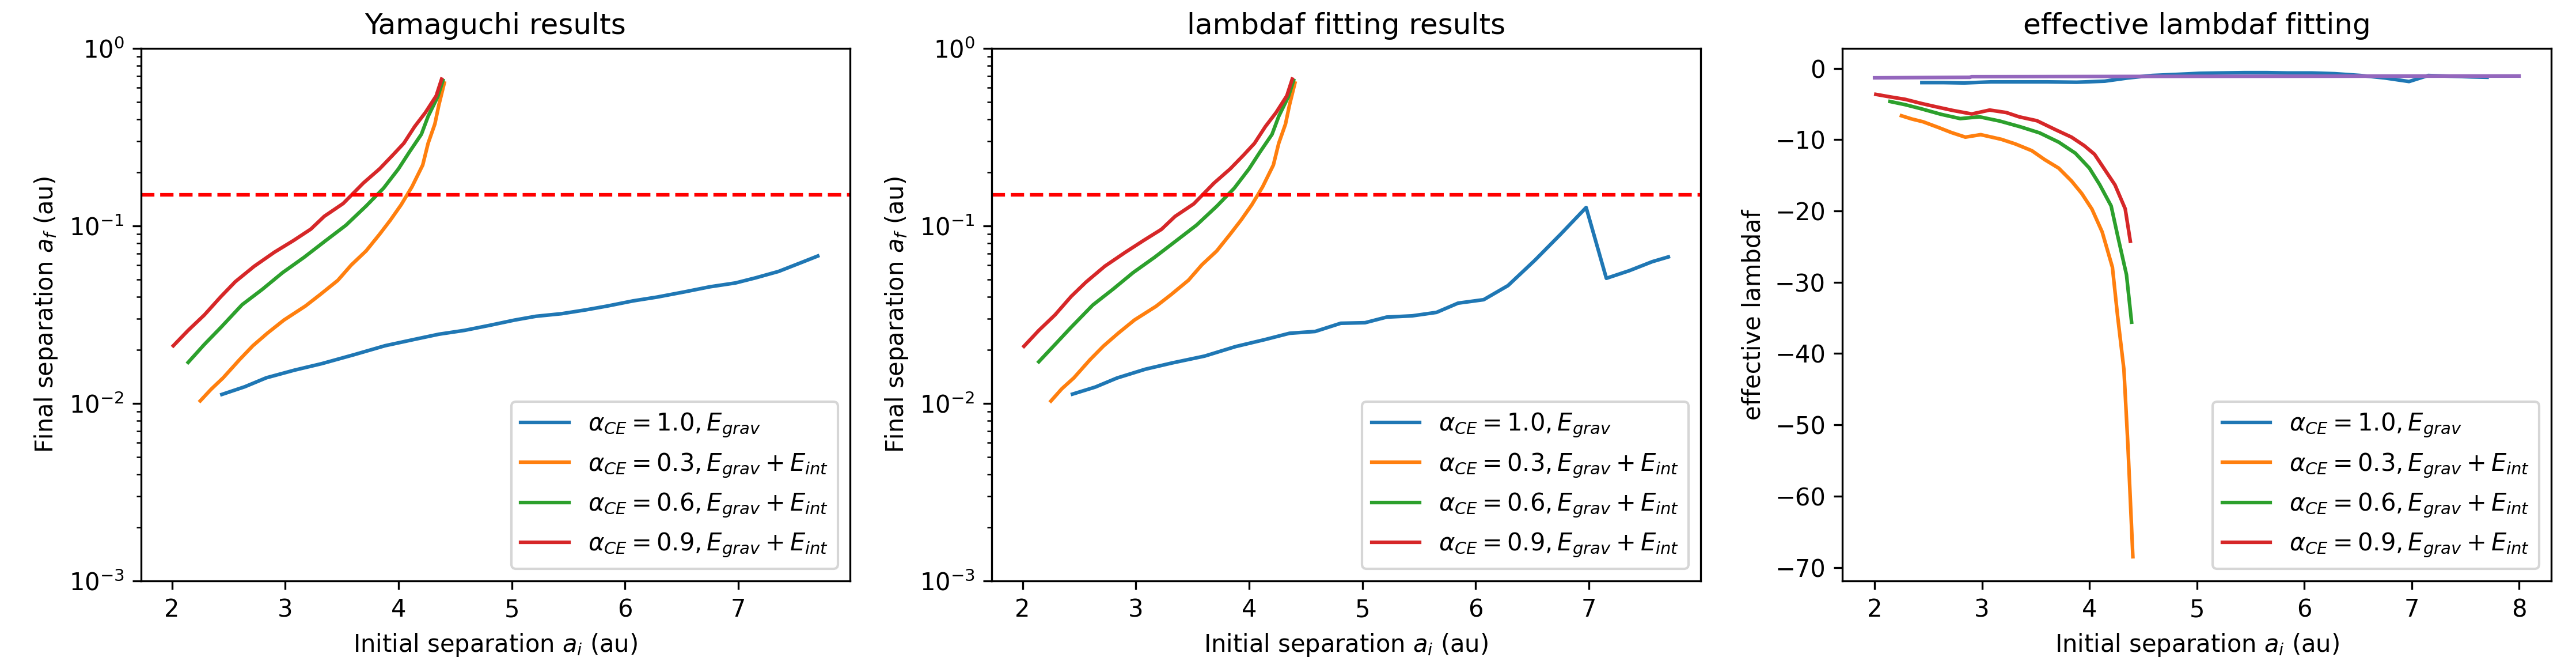
\includegraphics[width=\linewidth]{fig/7+1cmp.png}
  \caption{Same as Figure \ref{fit_hi}, but with default $\lambda$ in COSMIC model included in the right panel with the purple line.}
  \label{fit_cmp_hi}
\end{figure}

To further compare with the default $\lambda$ value in COSMIC, we include in the right panel an extra line which represents the default $\lambda$ value in COSMIC. This default $\lambda$ in the COSMIC model is calculated following Appendix A of \cite{claeys2014theoretical}. For all of our case, we have $M_{\mathrm{env}} > 1$. The results is shown in Figure \ref{fit_cmp_hi}. Notice that the default $\lambda$ value is at order $\sim 1$, far smaller than the effective $\lambda$ needed to recreate results in \cite{yamaguchi_hi}. Hence, we conclude that in COSMIC, it is not practical to form wide high mass WD+MS system through common envelope processes, since the required $\lambda$ is too large.

\begin{figure}
  \centering
  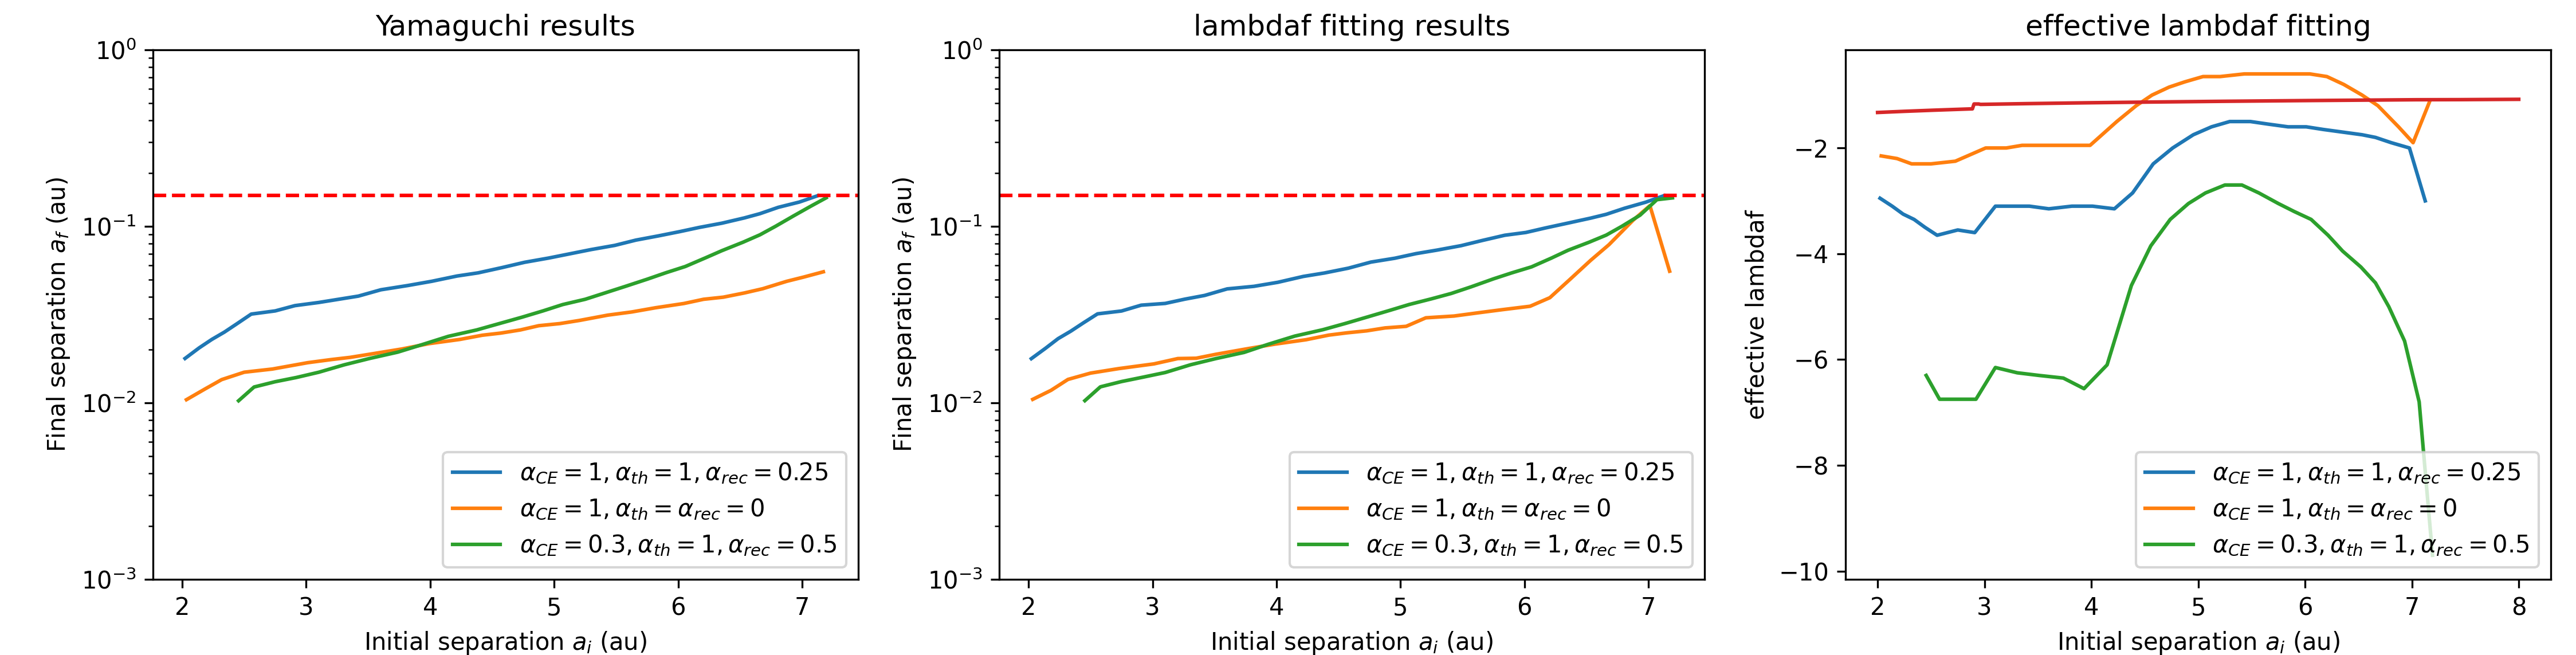
\includegraphics[width=\linewidth]{fig/7+1ebcmp.png}
  \caption{Same as Figure \ref{fit_cmp_hi}, but with a different common envelope energy budget. For results shown in these figures, $\Ebind = \Egrav + \alphath \Eth + \alpharec \Erec$, where the coefficients $\alphath$ and $\alpharec$ for different line is shown in the legend. The red line in the right panel indicates default $\lambda$ in COSMIC.}
  \label{fit_cmp_eb_hi}
\end{figure}

In Figure \ref{fit_cmp_eb_hi}, we present the same results for another energy budget of the CE process. Rather than including both thermal and recombination energy into the binding energy, we use two coefficients $\alphath$ and $\alpharec$ to consider their contribution to $\Ebind$ separately. That is,
\[
  \Ebind = \Egrav + \alphath \Eth + \alpharec \Erec.
\]
We notice that the effective $\lambda$ now gets with in the order of $\sim 10$. However, none of these initial separation and $\lambda$ results in wide WD+MS system with final separation $a_f > 0.15 \au$. Therefore, we conclude that with the new energy budget, it is not practical to form wide WD+MS binaries either.

\subsection{Low Mass Systems ($1.5 \Msun + 0.85 \Msun$)} \label{subsec:low}

\subsubsection{Methods and Results}
According to \cite{yamaguchi_lo}, the WD mass in the Gaia sample ranges from $0.5\Msun$ to $0.8\Msun$, which corresponds to progenitor mass of $1 \Msun$ to $3 \Msun$. The companions mass has a median of $0.85 \Msun$. MESA results for $1.5\Msun + 0.85\Msun$ systems is documented in \cite{yamaguchi_hi}. Hence, we consider a $1.5\Msun + 0.85\Msun$ evolution model in COSMIC and compare the results with those in \cite{yamaguchi_hi}. For the common envelope, we include all thermal energy $\Eth$ into the binding energy $\Ebind$, while the recombination energy $\Erec$ is included in part with a parameter $\alpharec$. That is,
\[
  \Ebind = \Egrav + \Eth + \alpharec \Erec.
\]

We take the same approach as high mass systems to investigate the effective value of $\lambda$ in COSMIC that matches with the results in MESA. The initial separation is a linear grid in range $0.5 \sim 6 \au$ with $400$ points. The CE flag \verb|lambdaf| is a linear grid in range $0 \sim -100$ with $2000$ steps, which corresponds to $0 \sim 100$ for CE parameter $\lambda$. Also, we ran these parameters with four different CE efficiencies — $\alphace = 1$, $\alphace = 0.9$, $\alphace = 0.6$, and $\alphace = 0.3$, the same as recorded in \cite{yamaguchi_lo}. In total, for each of the $4$ different CE efficiency $\alphace$, we ran a grid of $80000$ binary star systems with different initial separation $a_i$ and CE parameter $\lambda$.

After simulation is finished, we again select the time-step when the system finished CE for the first time, and record the final separation if the system is a desried WD+MS system. The result is presented in Figure \ref{res_lo}.

\begin{figure}
  \centering
  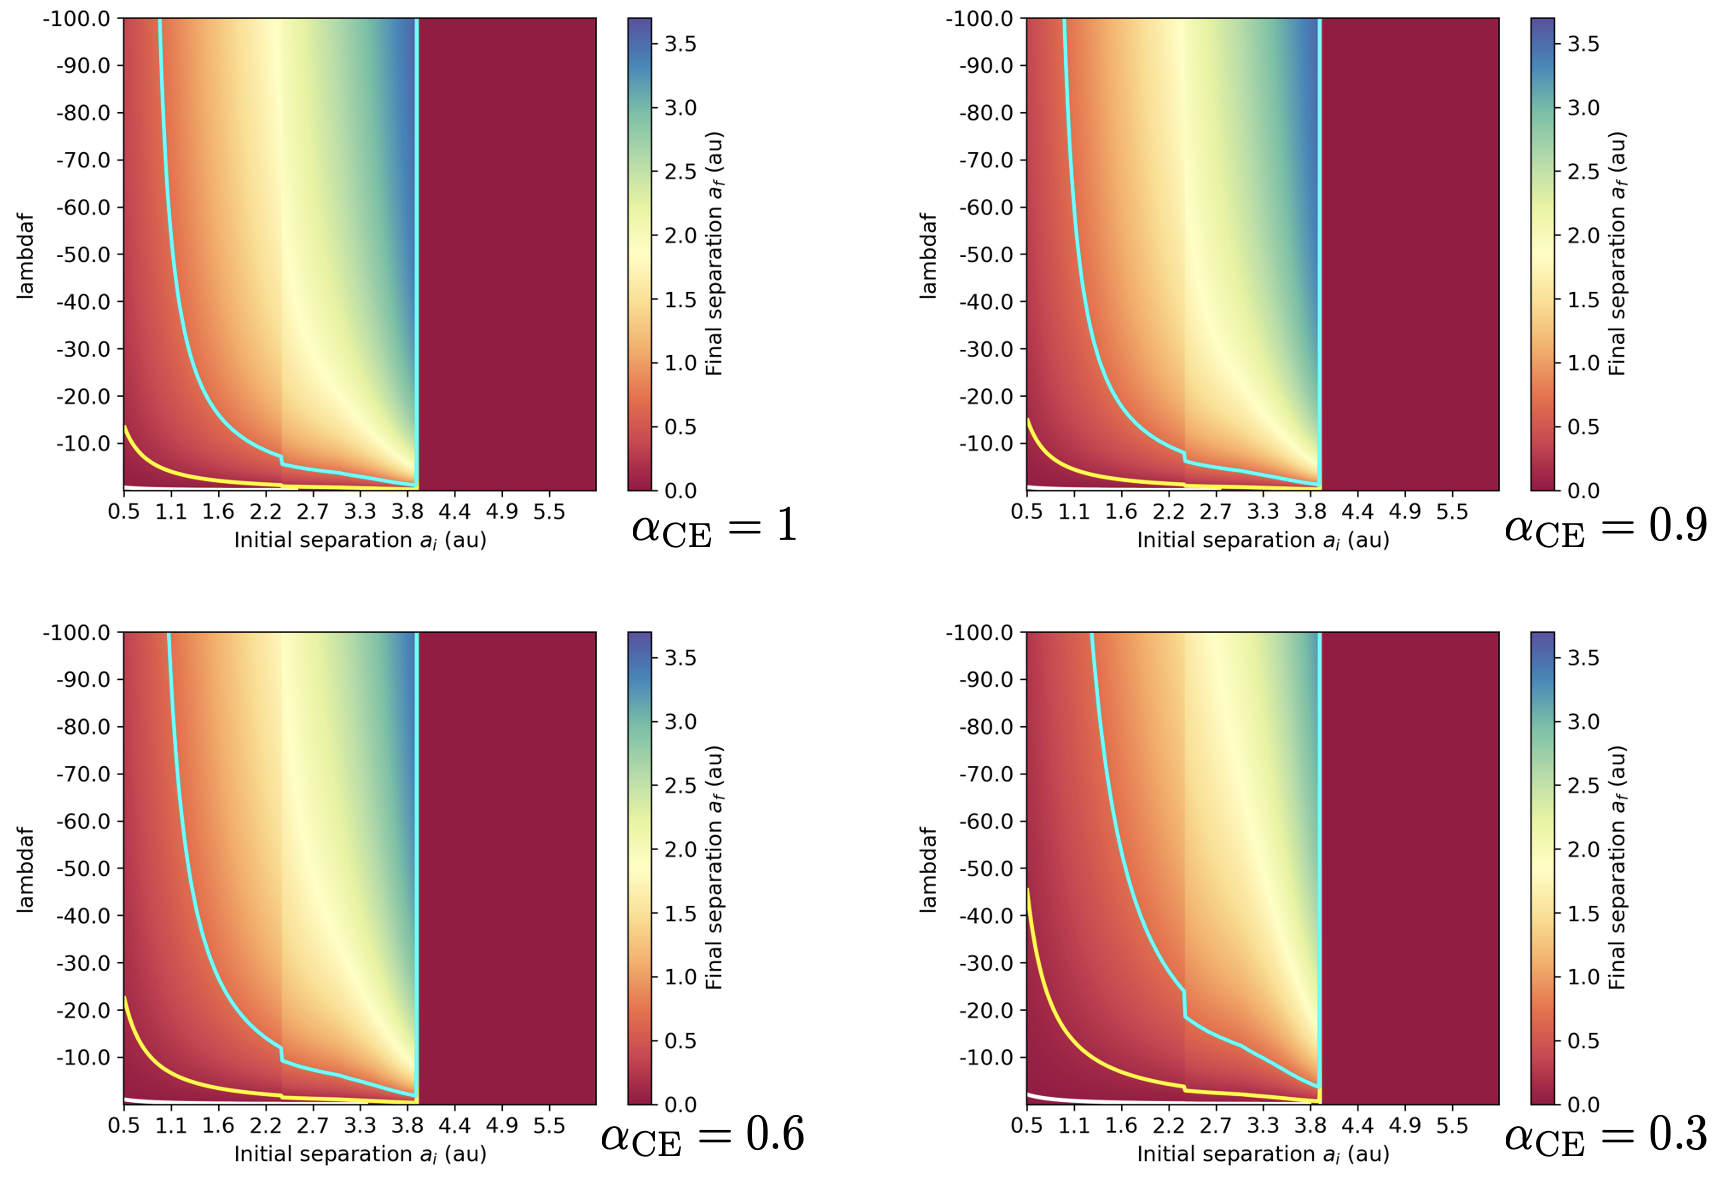
\includegraphics[width=\linewidth]{fig/1.5+0.8results.png}
  \caption{Heat map of final separation $a_f$ against initial separation $a_i$ and CE flag $-\lambda$. Different panels represent four different CE efficiencies $\alphace = 1$, $0.9$, $0.6$, and $0.3$. The white and yellow contour corresponds to $a_f = 0.01 \au$ and $a_f = 0.15 \au$ respectively. WD+MS binaries is not possible for separation smaller than $0.01 \au$, and $0.15 \au$ is the minimum separation of wide WD+MS binaries in observational results. Outside the white contour no desired system forms.}
  \label{res_lo}
\end{figure}

To compare the results with \cite{yamaguchi_lo}, we use the same approach as that for high mass systems. In Figure \ref{fit_cmp_lo_whole}, we compare COSMIC with MESA model that includes binding energy of the entire envelope. In Figure \ref{fit_cmp_lo_pt}, we compare COSMIC with MESA model that includes only binding energy of the outer envelope. Notice that we do not have fitting results for $a_i > 4 \au$. This is because no WD+MS binaries form in COSMIC for such initial separation range.

\begin{figure}
  \centering
  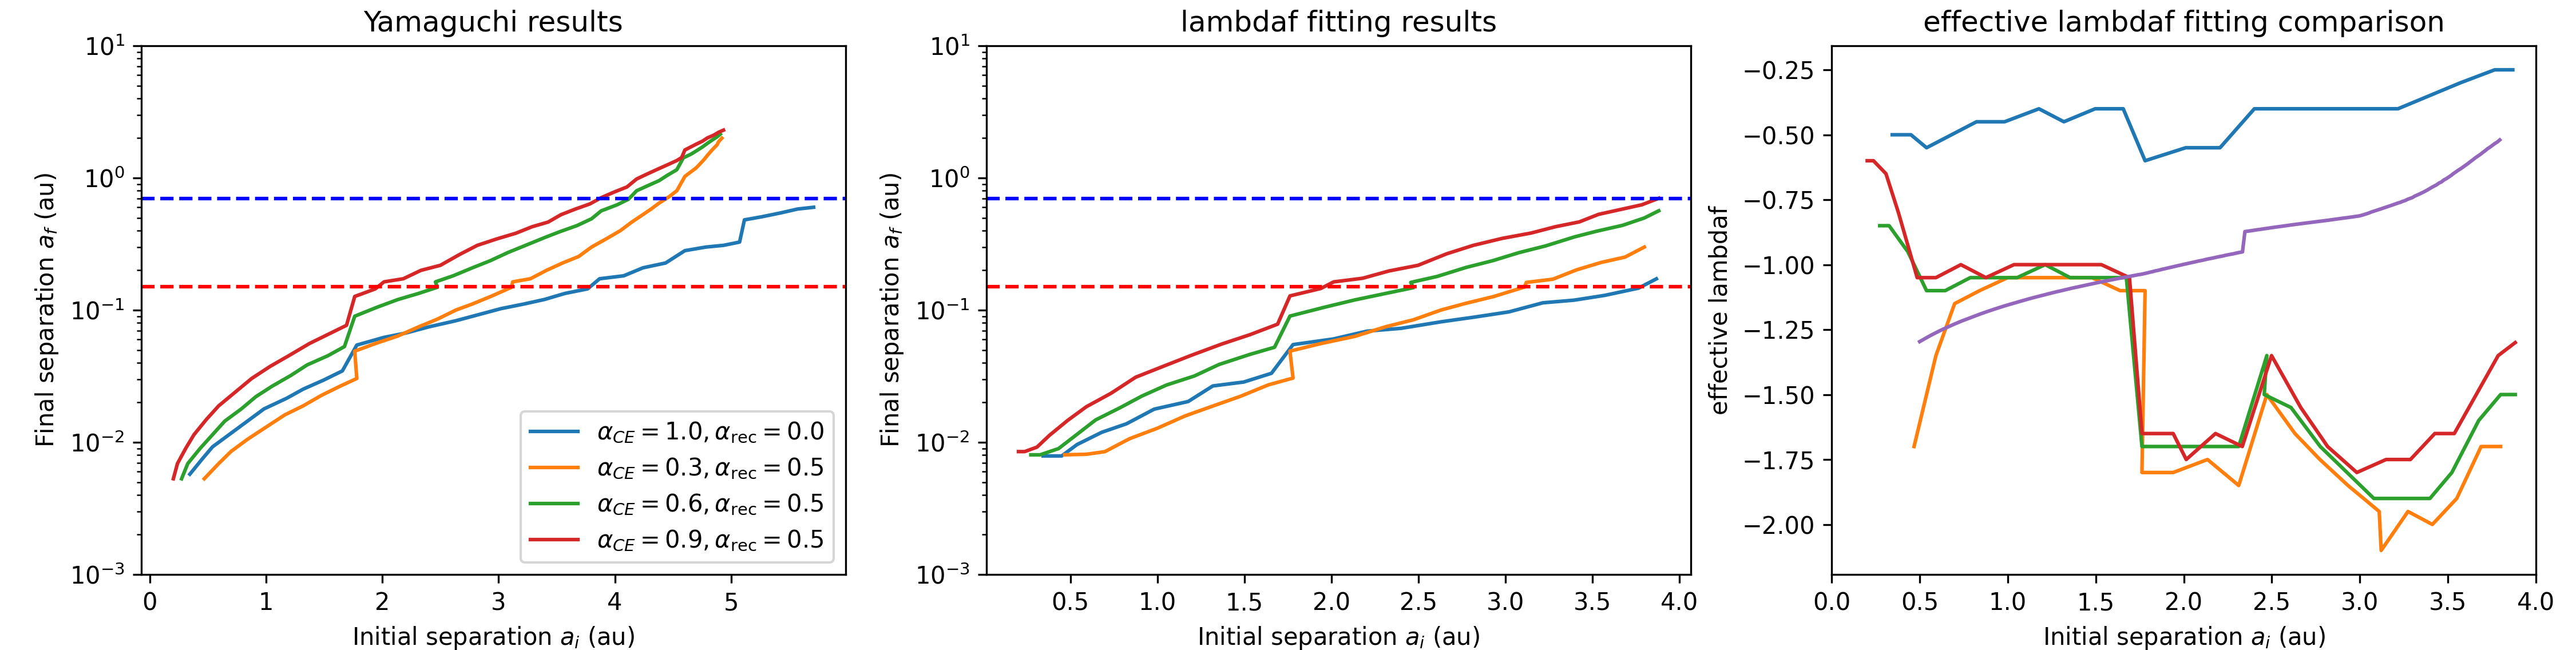
\includegraphics[width=\linewidth]{fig/1.5+0.8cmp_whole.png}
  \caption{Effective $\lambda$ fitting results of a $1.5\Msun + 0.85\Msun$ system for common envelope structure in MESA. Binding energy of the \emph{entire envelope} is considered. Left Panel: MESA results in \cite{yamaguchi_lo} of how final separation $a_f$ depends on initial separation $a_i$. Central Panel: COSMIC results of how final separation $a_f$ depends on initial separation $a_i$, produced by the effective $\lambda$. Right Panel: effective $\lambda$ in COSMIC that corresponds to the MESA results for each initial separation $a_i$. The purple line represents default $\lambda$ calculated using \cite{claeys2014theoretical}. The red dashed line and the blue dashed line in the left and central panel represents $0.15 \au$ and $0.7 \au$ respectively. $0.15 \au$ is the minimal separation for observed wide post-CE WD+MS binaries, while $0.7 \au$ is the typical separation for wide post-CE WD+MS binaries.}
  \label{fit_cmp_lo_whole}
\end{figure}

\begin{figure}
  \centering
  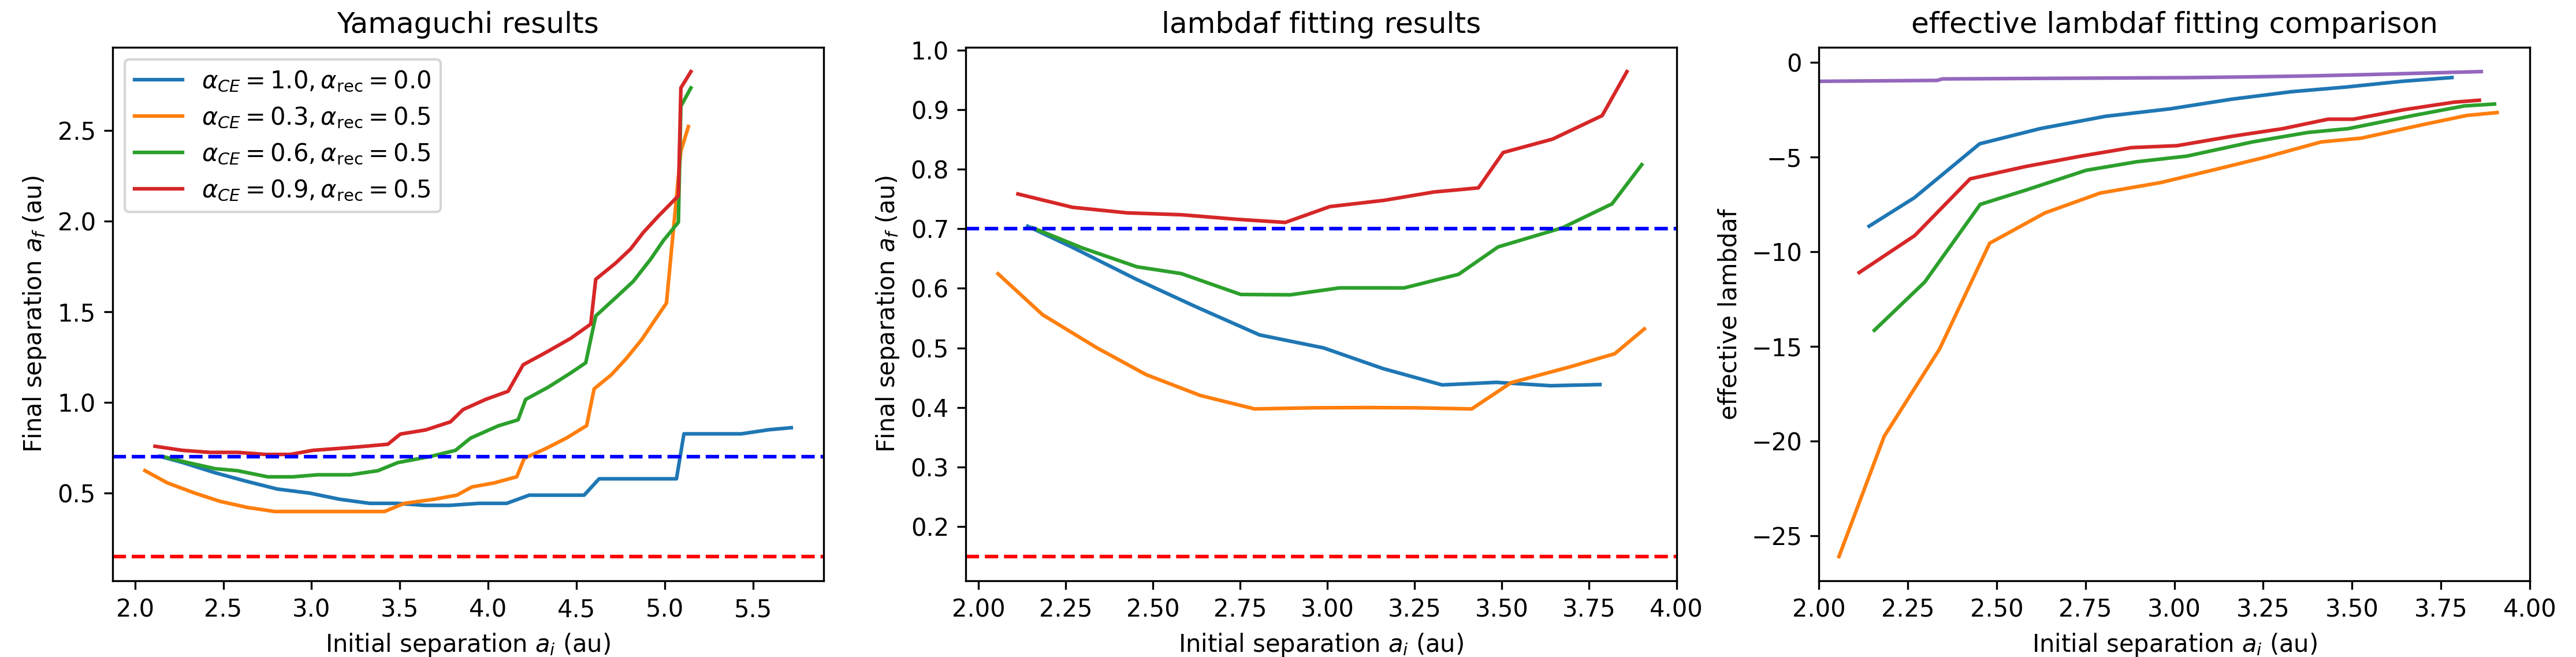
\includegraphics[width=\linewidth]{fig/1.5+0.8cmp_pt.png}
  \caption{Same as Figure \ref{fit_cmp_lo_pt} but only binding enregy of the \emph{outer envelope} is considered.}
  \label{fit_cmp_lo_pt}
\end{figure}

From the left panel of Figure \ref{fit_cmp_lo_whole}, we can see that wide WD+MS systems can form in MESA model when $a_i > 2.5 \au$. This is reproduced in COSMIC with $\lambda \sim 1$.Hence, wide WD+MS can form for $a_i > 2.5 \au$ with parameter $\lambda$ about the same as default. Recall that for high mass system, wide WD+MS systems cannot form without $\lambda \sim 10^2$. This is a significant difference between high mass systems and low mass systems.

\section{Formation Through Stable Mass Transfer} \label{sec:stable}

After exploring the formation of WD+MS binaries through common envelope, we investigate the possibility of forming WD+MS binaries through stable mass transfer. In \cite{yamaguchi_lo}, the author plot the $\MWD - \Porb$ relation of observed wide WD+MS bianries, and argues that it is not possible to form wide WD+MS binaries through stable mass. The plot is recreated in Figure \ref{theory-observed}, and from the figure, we can see that the observed wide post-mass transfer WD+MS bianries do not match the theoretical $\MWD - \Porb$ relation for stable mass transfer calculated in \cite{rappaport1995relation}. Also, the author aruges that stable mass transfer requires donors on SGB at the onset of mass transfer. However, this will not lead to WDs with masses observed \cite{yamaguchi_lo}. We will verfiy this idea in this section using $7\Msun + 1 \Msun$ binaries.

\begin{figure}
  \centering
  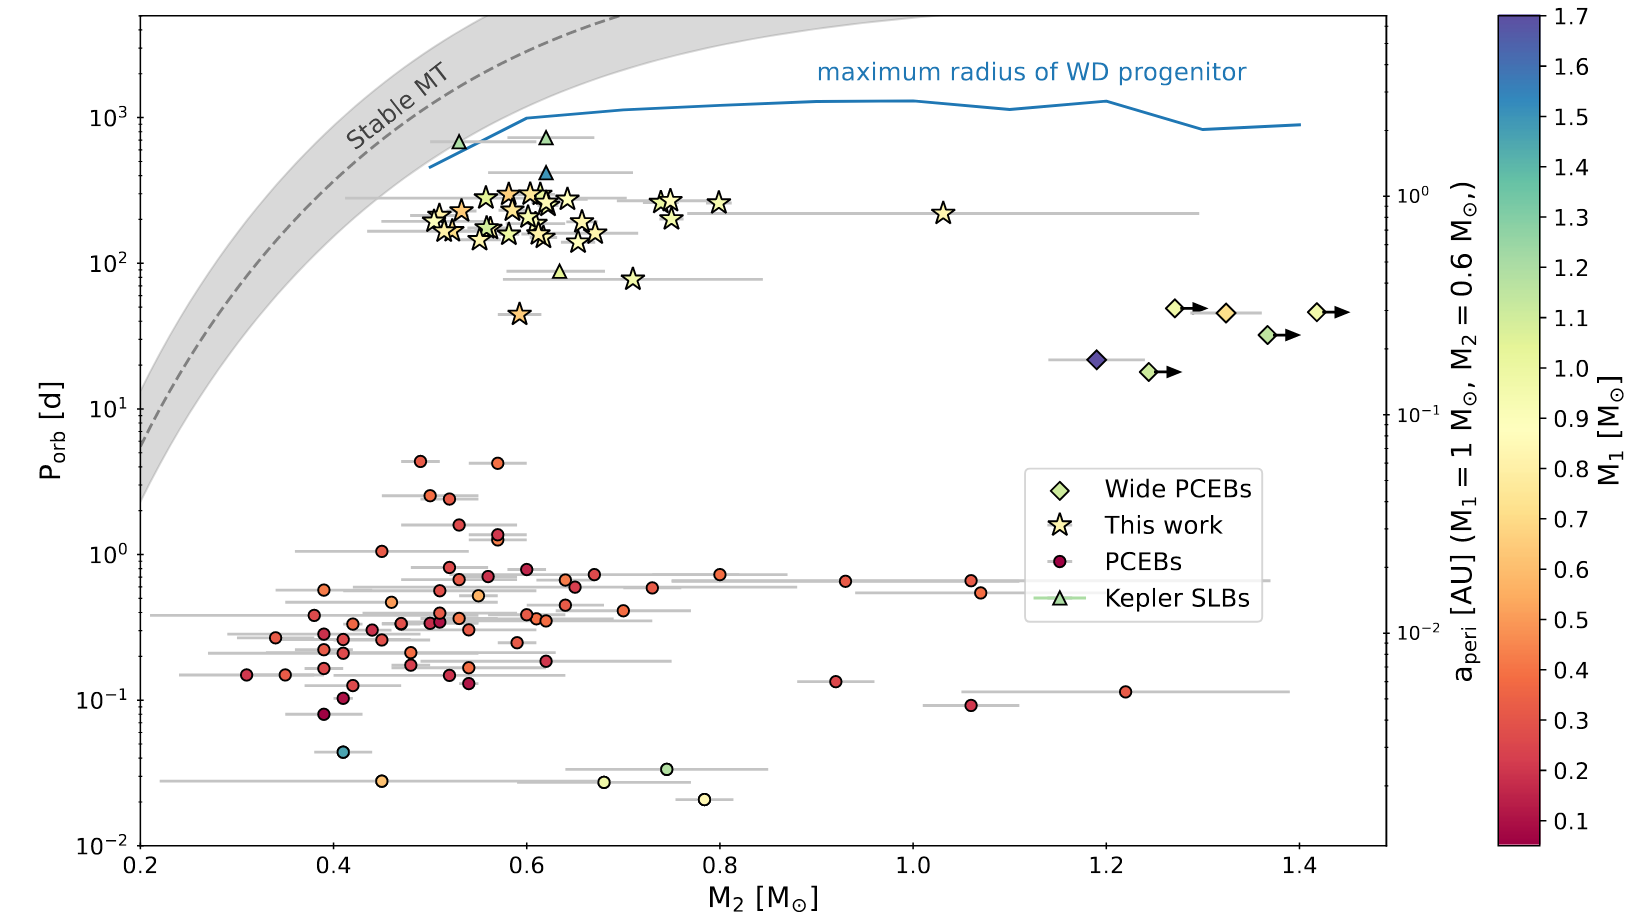
\includegraphics[width=0.8\linewidth]{fig/theory-observed.png}
  \caption{$M_{\mathrm{WD}} - P_{\mathrm{orb}}$ relation of observed wide post-mass transfer binaries. White dwarf mass $\MWD$ correspond to The colors of the points represent the masses of the luminous companion, $\Mstar$. On the right axis, we show the minimum orbital separation $a_{\mathrm{peri}}$, corresponding to the period assuming companion mass $\Mstar = 1 \Msun$ and white dwarf mass $\MWD = 0.6 \Msun$. The dashed line and the grey region is the track along which binaries undergoing stable MT are expected to evolve according to \cite{rappaport1995relation}}.
  \label{theory-observed}
\end{figure}

\subsection{Methods and Results}
First of all, to ensure stable mass transfer in COSMIC, we modify every entry of \verb|qcrit_array| in \verb|BSEDict| from the default $0.0$ to $20.0$. This changes the critical mass ratio for onset of unstable mass transfer to $20.0$ Based on our initial mass ratio $7:1$, this will make the actual mass raio of our system below this critical throughout the evolutionary process.

Secondly, a parameter on which stable mass transfer process depends is the accrection efficiency $\beta$, which in COSMIC is represented by \verb|acc_lim| in \verb|BSEDict|. Accretion efficiency is the fraction $\beta$ of all transfered materials that is accreted by the accretor. That is, $\dot{M_a} = -\beta\dot{M_d}$ where $M_d$ is the mass of donor and $M_a$ is the mass of accretor.

In our simulation, we investigate how accretion efficiency $\beta$ and initial separation $a_i$ affects the final separation $a_f$. We run a grid of three different accretion efficiency — $\beta = 0.0$, $0.5$ and $1.0$, and a linear grid of $a_i$ from $2 \au$ to $8 \au$ with $400$ steps. In total, we simulate $1200$ binaries with different accretion limit and initial separation. For each system, after the simulation is finished, we select the first timestep, if any, that shows a WD+MS binary. We record the separation at this moment as the final separation $a_f$, and we compare them with the observed minimum separation $0.15 \au$ for post-mass transfer WD binaries.

The results are presented in Figure \ref{stable_hi}. Notice the gap for $a_i$ ranges in $3 \sim 4.5 \au$. This means no WD+MS forms for this initial separation. In fact, for these initial separations and accretion efficiencies, two star merges.

\begin{figure}
  \centering
  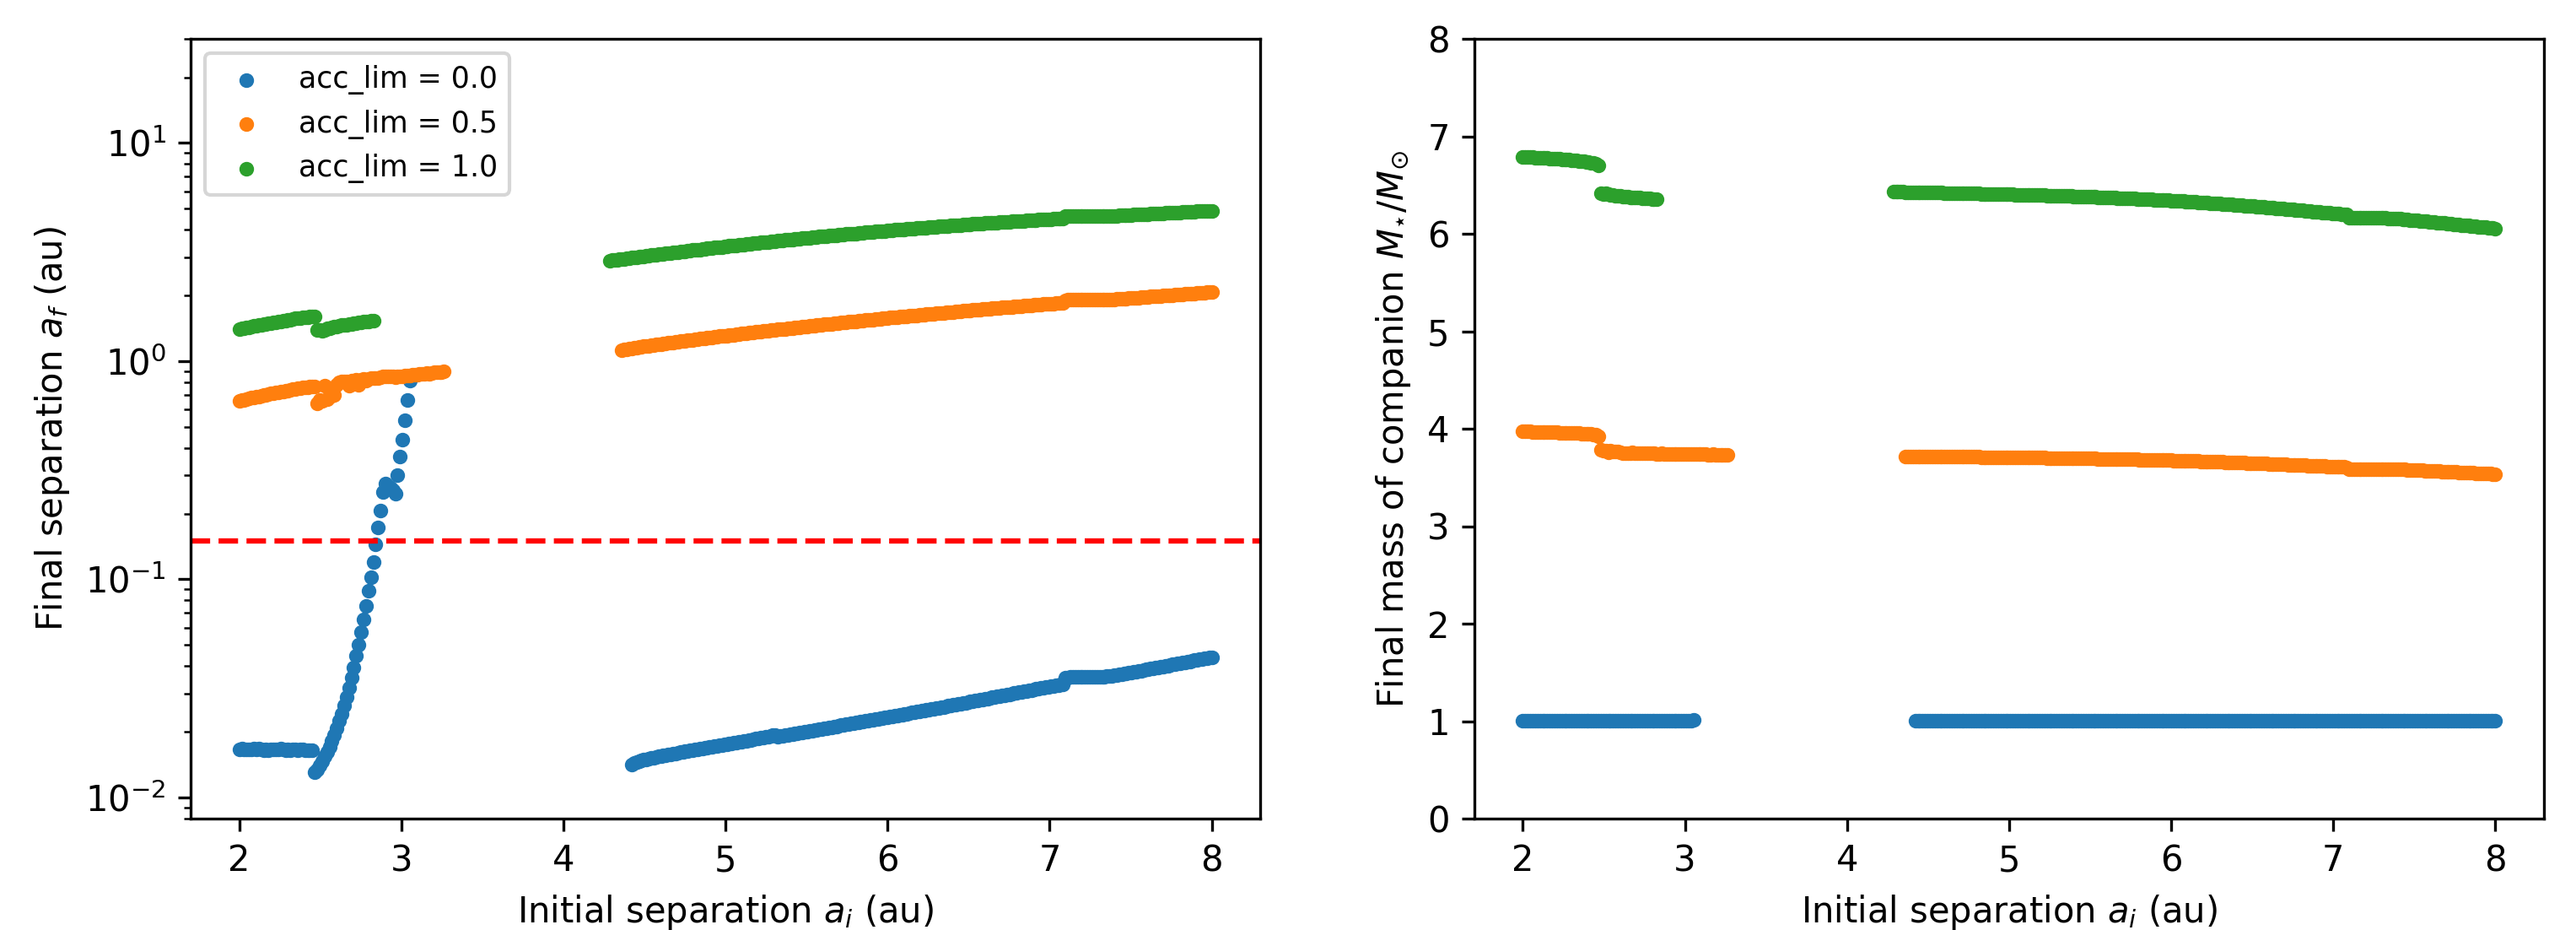
\includegraphics[width=0.75\linewidth]{fig/stable_hi_log.png}
  \caption{COSMIC results of WD+MS binaries after stable mass transfer for $7\Msun + 1\Msun$ systems, with accretion efficiency $\beta = 0$, $\beta = 0.5$, and $\beta = 1$ respectively. Left panel: dependence of final separation $a_f$ of the WD+MS binary on initial separation $a_i$. Right panel: the corresponding companion mass in solar units in the WD+MS binary. The gap in both figure represents that no WD+MS system forms for that initial separation.}
  \label{stable_hi}
\end{figure}

Notice that the majority of these systems have final separation $a_f > 0.15 \au$. However, this is \textbf{not the correct approach}, since the companion mass in our observed wide WD+MS binaries has median mass $\sim 1\Msun$. However, in the simulation results shown in Figure \ref{stable_hi}, the final companion mass is about $4 \Msun$ and $6.5 \Msun$ for $\beta = 0.5$ and $\beta = 1.0$ respectively. Hence, we need to adjust the  initial companion mass $M_{\star, i}$ and the accretion efficiency $\beta$, in order to make the final companion mass $M_{\star, f}$ close to $1\Msun$. Therefore, we lower the initial companion mass $M_{\star, i}$ and adjust the accretion efficiency $\beta$ and re-run the simulation. The results for $7\Msun + 0.7\Msun$ with $\beta = 0.1$, and $7\Msun + 0.5\Msun$ with $\beta = 0.2$ is shown in Figure \ref{stable_hi_ex}. 

After adjusting the initial mass of companion and the accretion efficiency, now the final mass of the companion is about $1\Msun$ and we get systems similar to our observed samples. 
Also, in Figure \ref{stable_hi_ex}, we note that when initial separation $a_i$ lies in the range of $2.5 \sim 4.5 \au$, the final separation incerases sharply. Also, it is only in this region that $a_f$ goes larger than the observed minimum $0.15 \au$ for wide WD binaries. Hence, in the next subsection, we will try to explain this sharp increases qualitatively.

\begin{figure}
  \centering
  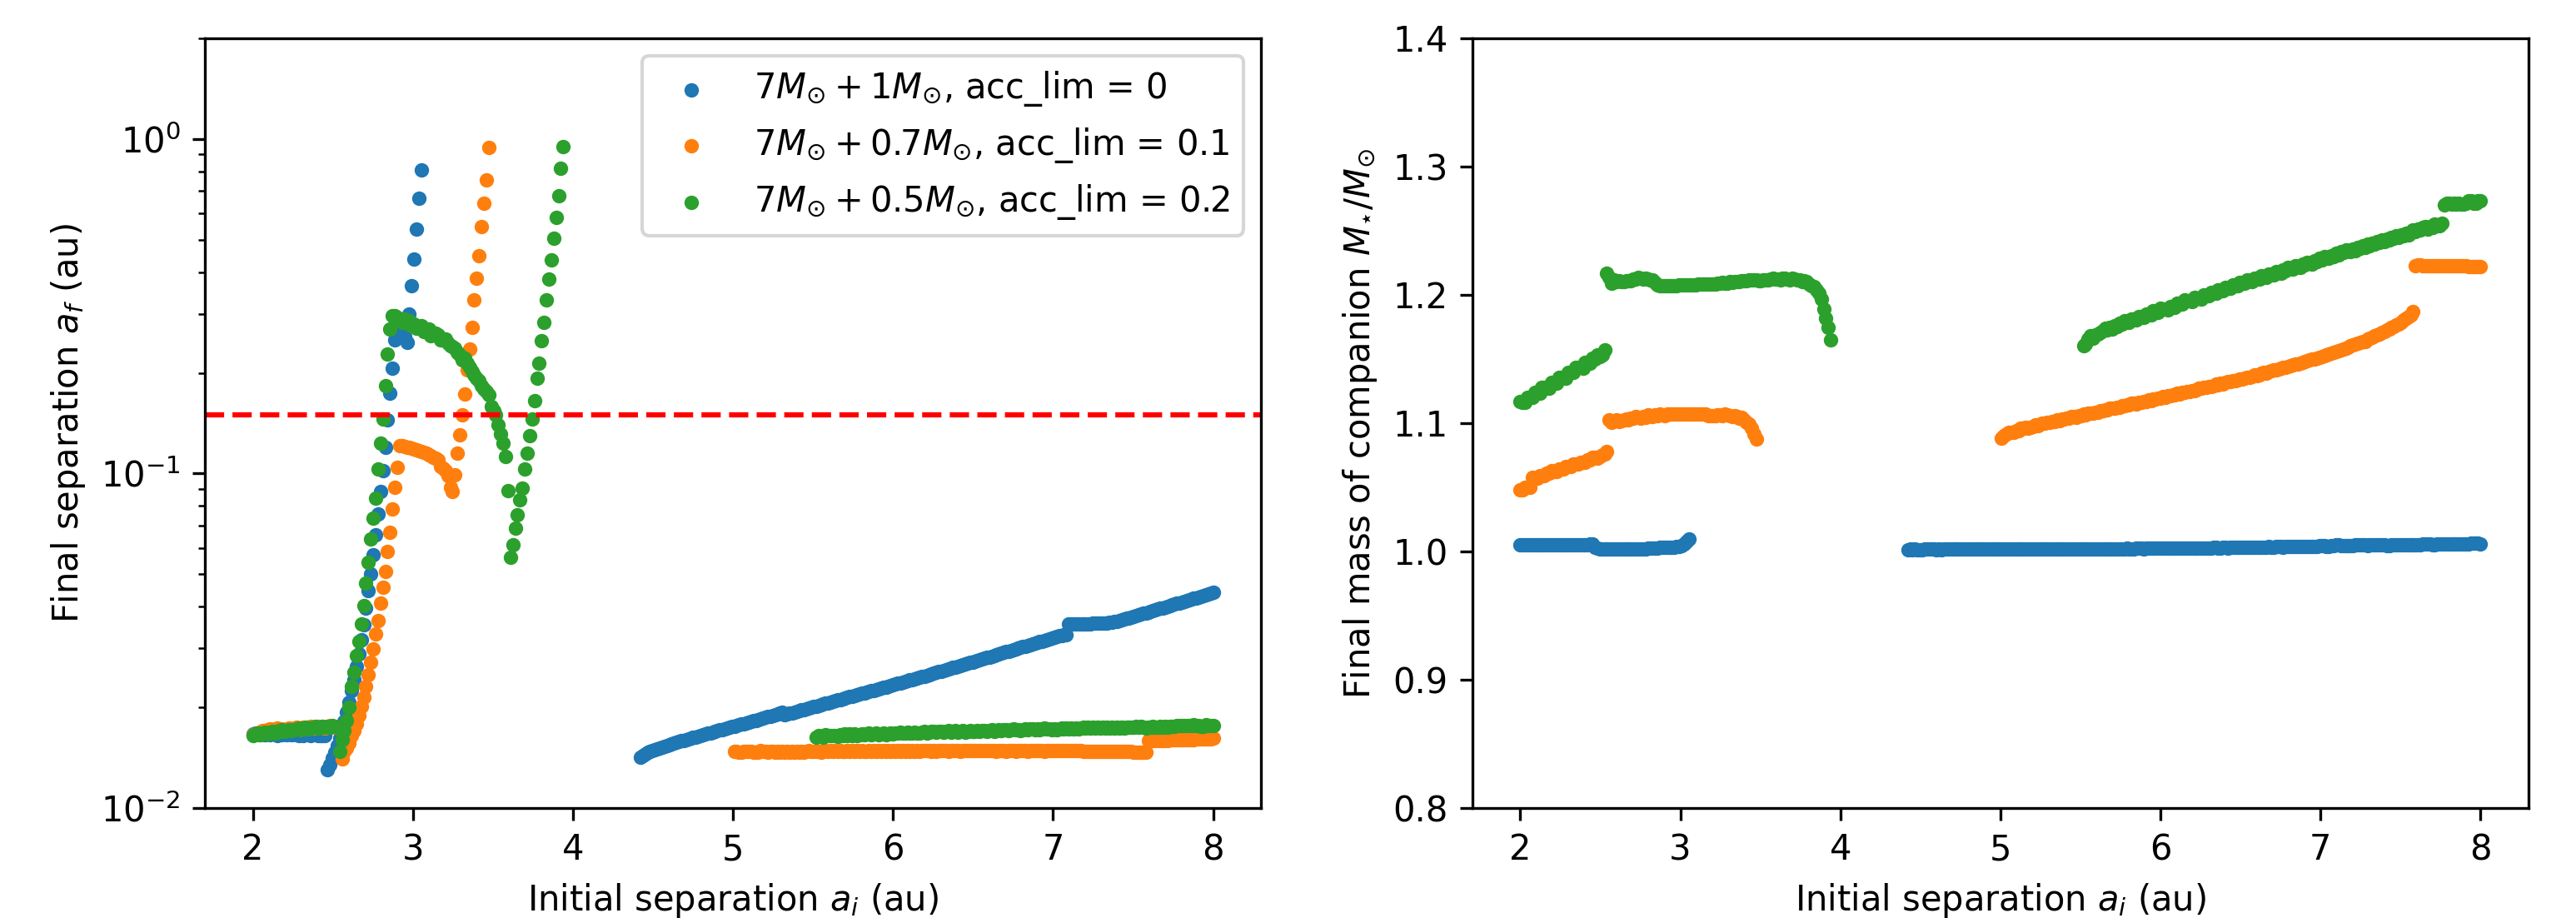
\includegraphics[width = 0.75\linewidth]{fig/stable7+1ex.png}
  \caption{COSMIC results of WD+MS binaries after stable mass transfer for two systems — $7\Msun + 0.7\Msun$ with accretion efficiency $\beta = 0.1$, and $7\Msun + 0.5\Msun$ with accretion efficiency $\beta = 0.2$. The left and right panel presents the same content as in Figure \ref{stable_hi}.}
  \label{stable_hi_ex}
\end{figure}

\subsection{Discussions}
In the previous section, we mentioned how $7\Msun + 1 \Msun$ systems with $\beta = 0$, $7 \Msun + 0.7\Msun$ systems with $\beta = 0.1$, and $7 \Msun + 0.5 \Msun$ systems with $\beta = 0.2$ produces WD+MS binaries with final separation $a_f > 0.15 \au$ and companion mass $\sim 1 \Msun$ in certain range of $a_i$.

From figure \ref{stable_hi_ex}, we can see that the dependence of $a_f$ on $a_i$ can be roughly divided into four parts. The \textbf{pre-spike} part before the sharp increase with $a_i < 2.5 \au$, the \textbf{spike} part where the $a_f$ inrceases sharply with $2.5 \au < a_i < 3.5 \au$, the gap where the two stars merge with $3.5 \au < a_i < 4.5 \au$, and the part after that with $a_i > 4.5 \au$.

Typical \textbf{pre-spike} and \textbf{spike} systems both follows the evolution path $\boxed{\text{\textbf{*-3-*-5-7-8-4-*-3-*-4-*}}}$ before reacing WD+MS. Note that the binaries come into contact (\verb|evol_type = 5|), which follows by a common enevelope phase. After inspecting the evolutionary process more closely, we found that the second stable mass transfer tends to widens the orbit significantly. \textbf{(***TO-DO***)}

\section{Population Synthesis Results} \label{sec:population}
After investigating how the final separation depends on various parameters in individual binary star systems, we now shift our focus onto the distribution of final orbital period in a population of binaries (equivalent to final separation since $\Porb^2 \sim a^3$).

\subsection{Methods}
First of all, we sample the binary population using the independent sampler in COSMIC. We set the primary mass model to \verb|korupa01|, eccentricity model to \verb|uniform|, and orbital period model, together with the binary fraction model to \verb|moe19|. We sample a total number of about $10000$ binaries with solar metallicity. The distribution of primary mass and the orbital period in the sampled population is shown in the Figure \ref{sample-distribution}.

\begin{figure}
  \centering
  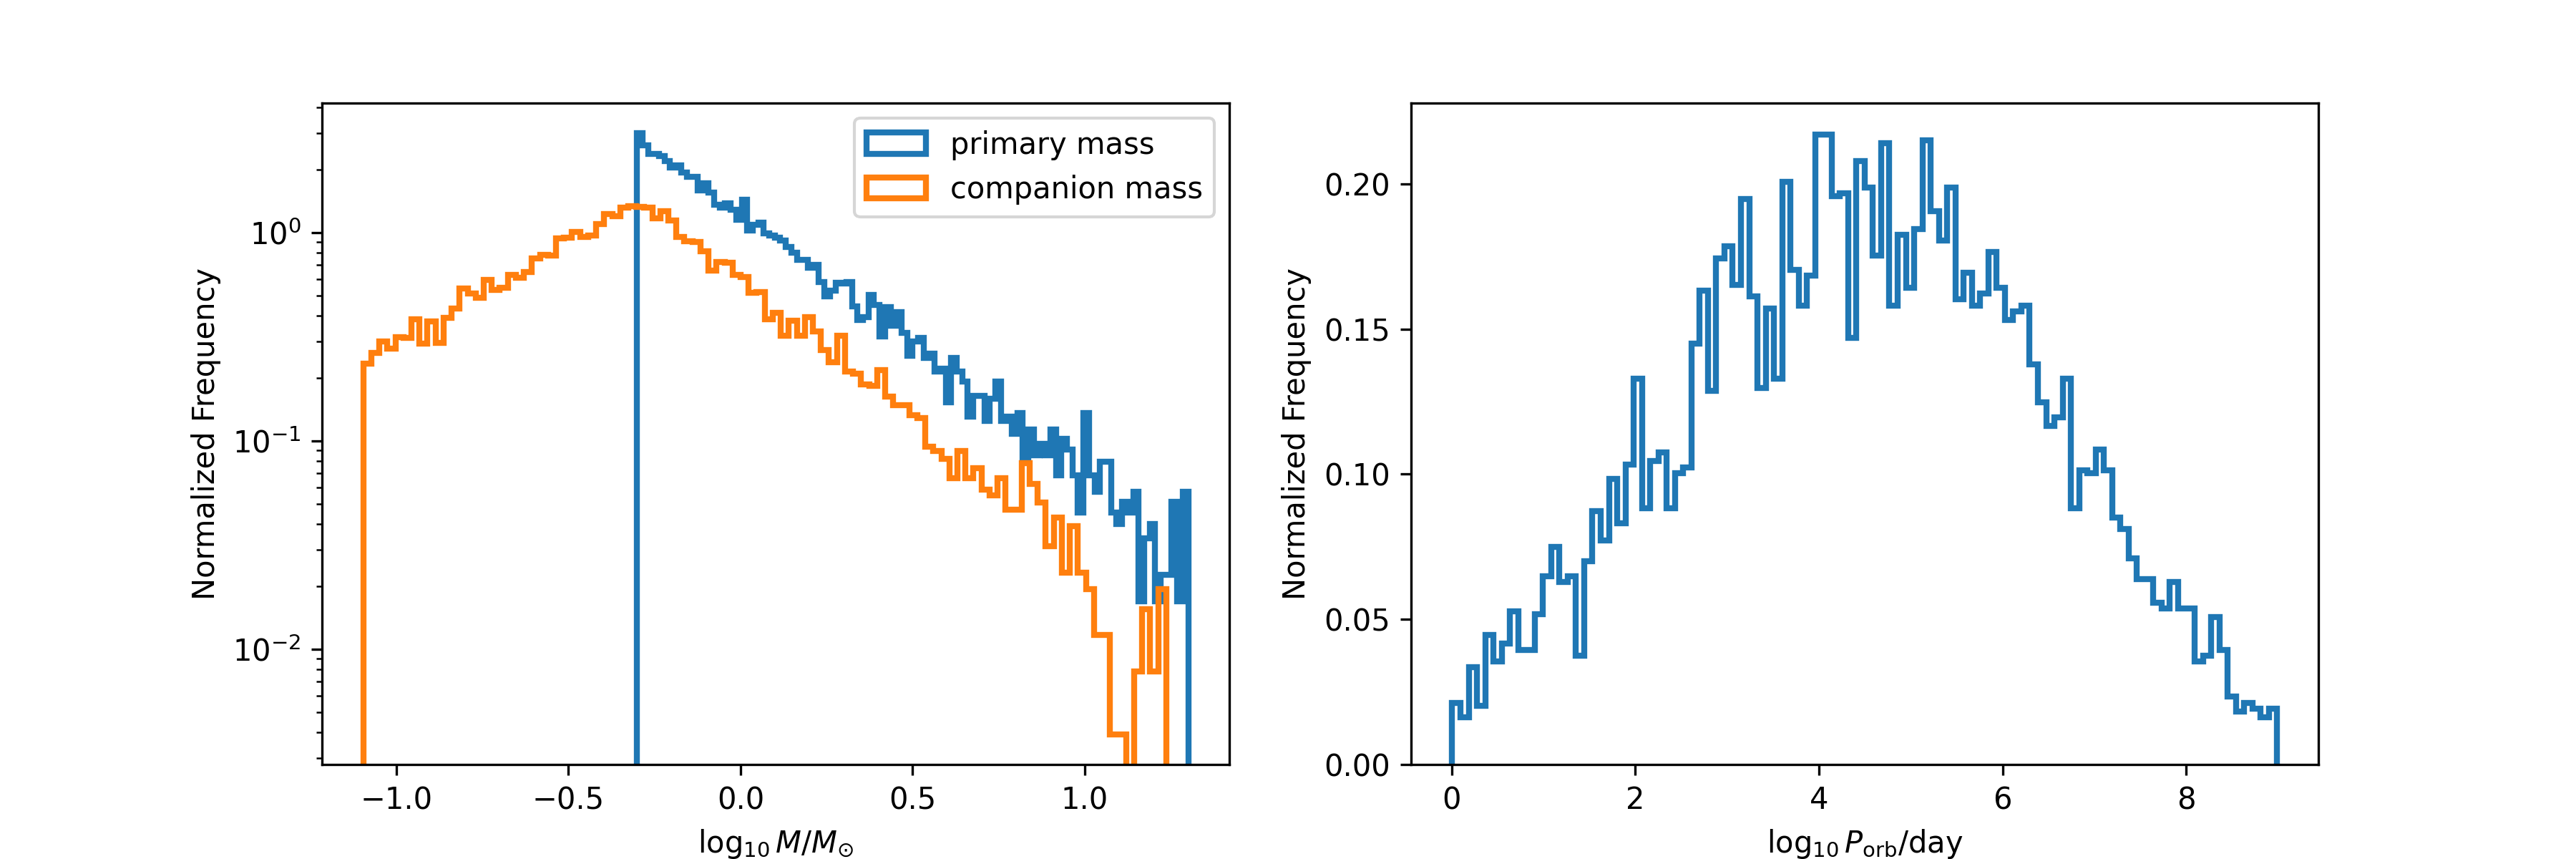
\includegraphics[width=\linewidth]{fig/sample-distribution.png}
  \caption{The distribution of primary mass, companion mass, and orbital period in the sampled population using independent sampler. Left panel: distribution of primary mass and companion mass in log scale. Right panel: distribution of orbital period $\Porb$ in log scale.}
  \label{sample-distribution}
\end{figure}

To investigate how the final white dwarf mass and orbital period depends on \verb|lambdaf|, we simulation the same sampled population with five different $\lambda$ values, $\lambda = 5$, $15$, $25$, $35$, $45$. After that, we select the first time-step that satisfies \verb|evol_type = 8|, \verb|kstar_1| is WD, and \verb|kstar_2| is MS. We record the white dwarf mass $\MWD$ and the final orbital period $P_{\mathrm{orb}, f}$ from this moment. We also select the moment when the first Roche lobe overflow starts, and record the initial orbital separation $P_{\mathrm{orb}, i}$ and \verb|kstar_1| type at this moment. These variables will later help us study how the orbit widens, with respect to different parameter $\lambda$ and initial separation $a_i$.

\subsection{Results}
\begin{figure}
  \centering
  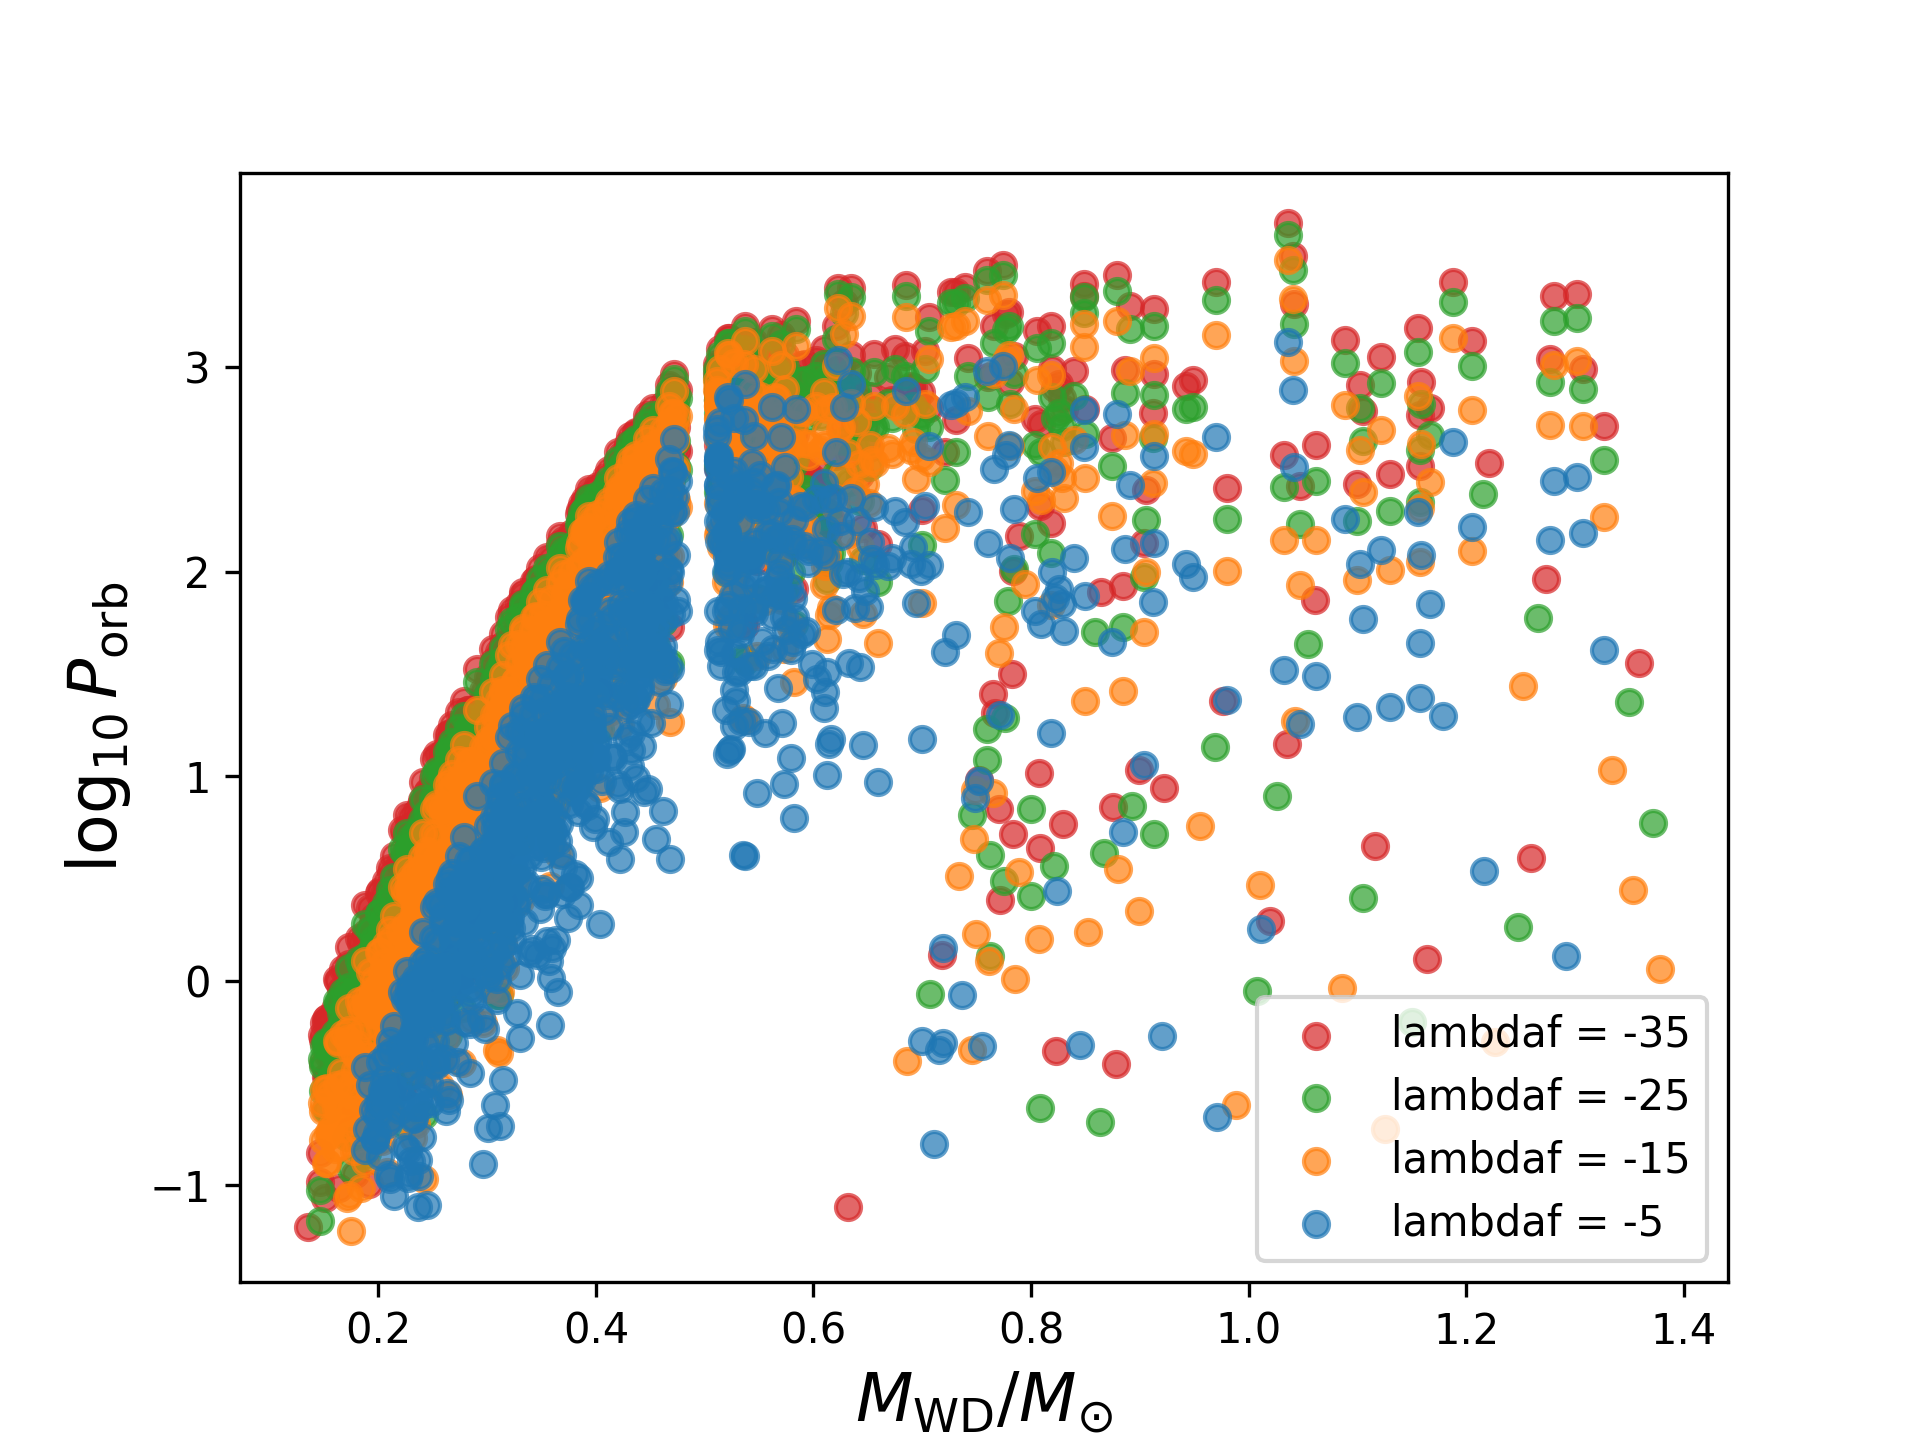
\includegraphics[width=0.6\linewidth]{fig/Mwd-P scatter.png}
  \caption{Scatter plot of white dwarf mass $\MWD$ and final orbital period after common envelope in log scale $\log_{10}\Porb$. Different colors indicates results for different $\lambda$ values. For each different $\lambda$ value the same initial population is used.}
  \label{Mwd-P-scatter}
\end{figure}

To show how the change in $\lambda$ affects the final orbital period, we plot final orbital period $\Porb$ against white dwarf mass $\MWD$ in Figure \ref{Mwd-P-scatter}. From Figure \ref{Mwd-P-scatter}, we note that the final orbital period is larger in general for larger $\lambda$. This can be clearly seen from the figure for $\MWD$ ranges in $0.2 \sim 0.7 \au$. This is also expected based on Equation \ref{ebind}, since for larger $\lambda$, less energy is required to unbind the common envelope, leading to more energy after mass transfer and a larger orbital period.

\begin{figure}
  \centering
  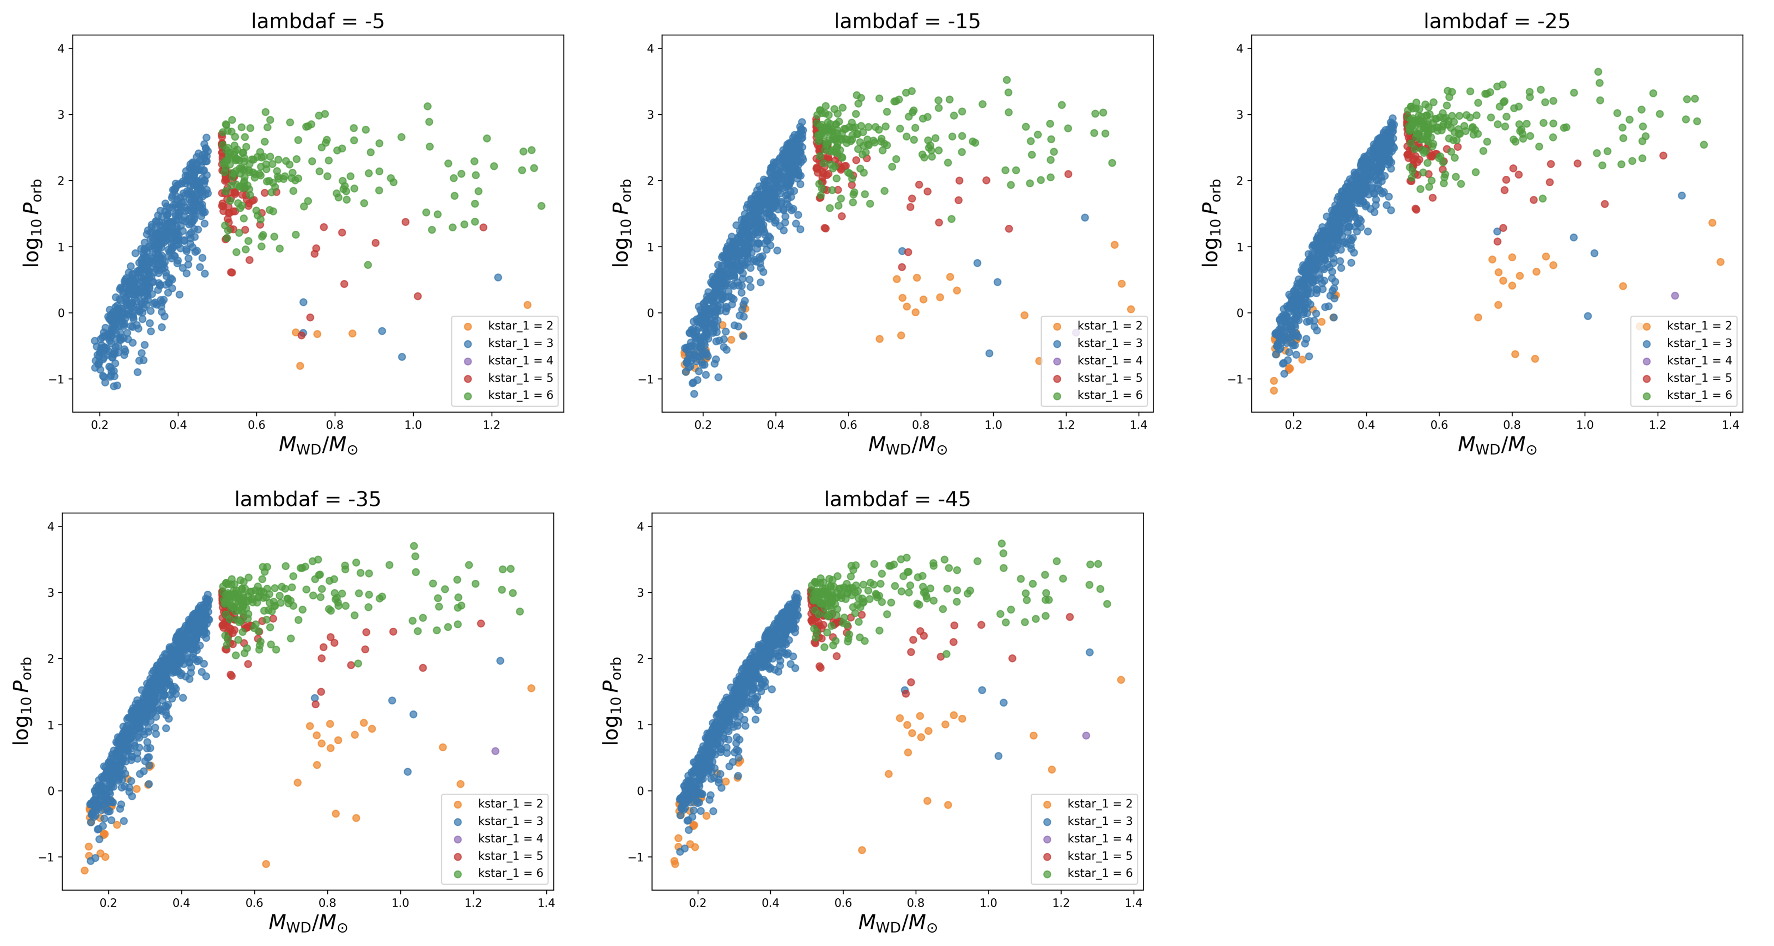
\includegraphics[width=\linewidth]{fig/kstar-map-rearr.png}
  \caption{Each panel: for this $\lambda$ value in the title, scatter plot of white dwarf mass $\MWD$ and final orbital period after common envelope in log scale $\log_{10}\Porb$. Different colors represent different kstar type of the primary at the start of mass transfer.}
  \label{kstar-map}
\end{figure}

To also show how the final separation $\Porb$ depends on \verb|kstar_1| type at the start of first RLOF, we plot $\Porb$ against $\MWD$ for different $\lambda$ separately, and use different color to distinguish between different \verb|kstar_1| type at the start of mass transfer. The plot is shown in Figure \ref{kstar-map}. In general, if the star is at later stages of evolution (larger \verb|kstar|) when mass transfer starts, then the resulting white dwarf mass $\MWD$ and $\Porb$ are also both larger. Note also that few systems start the mass transfer at \verb|kstar_1 = 2| (Hertzsprung gap) and \verb|kstar_1 = 4| (Core Helium Burning). This is because stars crosses Hertzsprung in a short timescale, leaving little time for interaction. Also, stellar radius is small when going through Core Helium Burning, reducing the possibility of interactions that starts when \verb|kstar_1 = 4|.

\begin{figure}
  \centering
  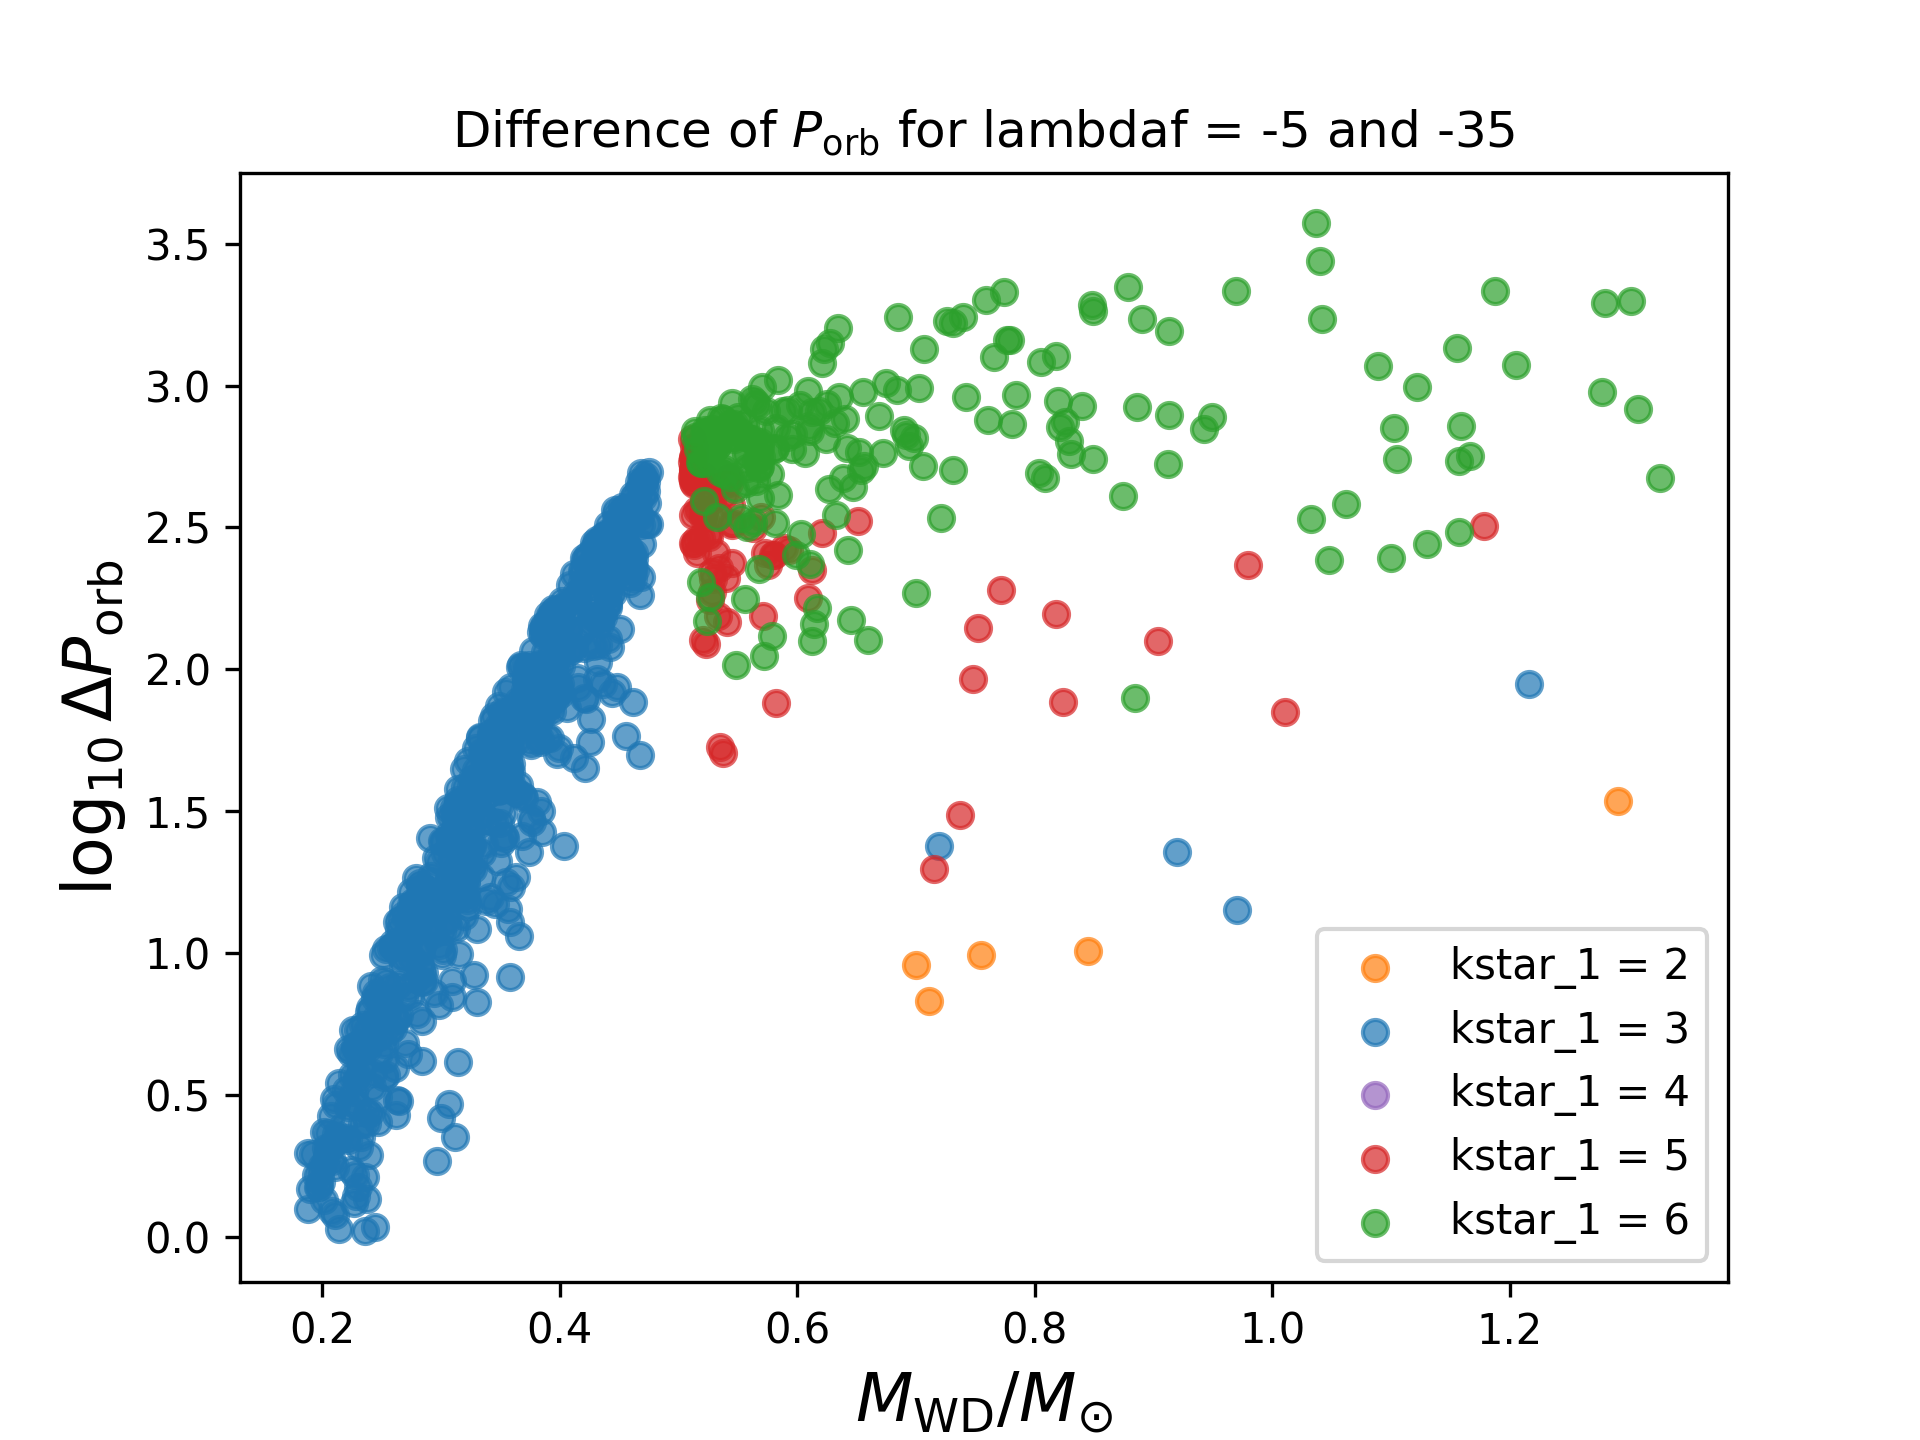
\includegraphics[width=0.6\linewidth]{fig/dif-kstar map.png}
  \caption{Scatter plot of difference in orbital period $\Delta P = P_{\mathrm{orb}}^{\lambda = 35} - P_{\mathrm{orb}}^{\lambda = 5}$ against the white dwarf mass $\MWD$. Different colors indicates different kstar type of the primary at the start of mass transfer.}
  \label{dif-kstar map}
\end{figure}

\begin{figure}
  \centering
  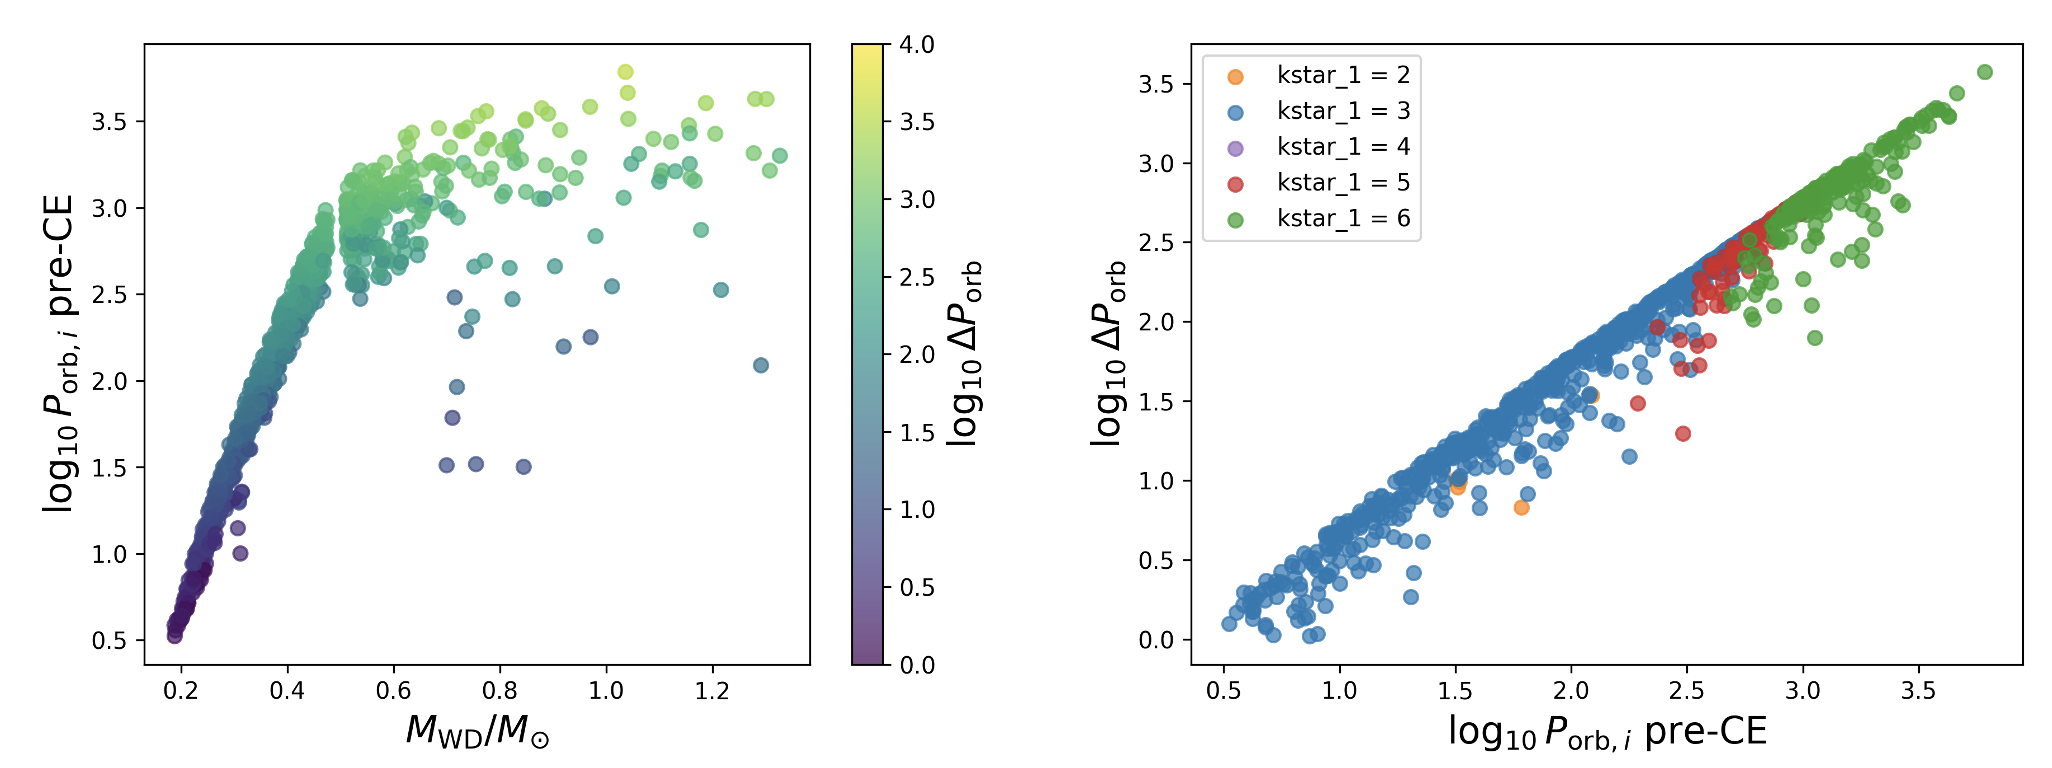
\includegraphics[width=\linewidth]{fig/dif-kstar two plot.png}
  \caption{Left panel: scatter plot of initial orbital period at the start of RLOF $P_{\mathrm{orb}, i}$ against the final white dwarf mass $\MWD$. The color of the dots indicates how the final orbital period $P_{\mathrm{orb}, f}$ changes with respect to $\lambda=35$ and $\lambda=5$. That is, the color indicates the magnitude of $\Delta P = P_{\mathrm{orb}}^{\lambda = 35} - P_{\mathrm{orb}}^{\lambda = 5}$. Right panel: scatter plot of $\log_{10} \Delta \Porb$ against the initial orbital period in log scale $\log_{10} P_{\mathrm{orb}, i}$ at the start of RLOF. Different colors indicates different kstar type of the primary at the start of RLOF.}
  \label{dif-kstar-exp}
\end{figure}

To visualize the difference in final orbital period $\Porb$, and how they corresponds to different \verb|kstar_1| type at the start of RLOF, we create plot the difference in orbital period $\Delta P = P_{\mathrm{orb}}^{\lambda = 35} - P_{\mathrm{orb}}^{\lambda = 5}$ against the white dwarf mass $\MWD$ in Figure \ref{dif-kstar map}. From Figure \ref{dif-kstar map}, we can see that for large \verb|kstar_1| type at the start of RLOF, $\Delta P = P_{\mathrm{orb}}^{\lambda = 35} - P_{\mathrm{orb}}^{\lambda = 5}$ is also larger. To explain this, we plot the how final white dwarf mass $\MWD$, difference in final orbital period $\Delta \Porb$, and orbital period before mass transfer $P_{\mathrm{orb}, i}$ related to each other in Figure \ref{dif-kstar-exp}. We see that the larger initial orbital period $P_{\mathrm{orb}, i}$, the more significant effect does $\lambda$ have on the final orbital period. This is not unexpected since during mass transfer, the separation changes as $\dot{a} / a = \text{const}$. Hence $\dot{\Porb} / \Porb = \text{const}$. Therefore, the larger the initial orbital period, the larger it changes, and thus the larger effect does $\lambda$ have.

\newpage
\bibliography{reference.bib}
\bibliographystyle{apalike}

\end{document}

